% =====================================================================
% SeaNergy - IEEE-style conference manuscript
% Hyper Grey, Smart India Hackathon 2026, problem statement 26058
% Build: xelatex SeaNergy_Adaptive_Sonar_Research_Paper.tex (twice)
% =====================================================================
\documentclass[conference,a4paper]{IEEEtran}
% SeaNergy technical report - shared preamble.
% Kept separate so appendices can be built standalone against the same styling.

\usepackage{fontspec}
\setmainfont{Times New Roman}
\usepackage{microtype}
\usepackage{amsmath,amssymb}
\usepackage{siunitx}
\usepackage{graphicx}
\usepackage{booktabs}
\usepackage{tabularx}
\usepackage{longtable}
\usepackage{array}
\usepackage{float}
\usepackage{xcolor}
\usepackage{fancyhdr}
\usepackage{enumitem}
\usepackage[hidelinks]{hyperref}

% ---------------------------------------------------------------- palette
\definecolor{ink}{HTML}{111820}
\definecolor{ocean}{HTML}{136578}
\definecolor{teal}{HTML}{1E8C9E}
\definecolor{rule}{HTML}{C8D2D8}
\definecolor{soft}{HTML}{F2F6F7}

% ---------------------------------------------------------------- units
\sisetup{
  detect-all,
  range-phrase = {\,--\,},
  range-units = single,
  group-separator = {,},
  per-mode = symbol,
}
\DeclareSIUnit{\NTU}{NTU}
\DeclareSIUnit{\ppt}{ppt}
\DeclareSIUnit{\dBc}{dBc}
\DeclareSIUnit{\Sps}{Sps}
\DeclareSIUnit{\dBFS}{dBFS}

% ---------------------------------------------------------------- headers
\pagestyle{fancy}
\fancyhf{}
\renewcommand{\headrulewidth}{0pt}
\renewcommand{\footrulewidth}{0pt}
\fancyhead[L]{}
\fancyhead[R]{\footnotesize Hyper Grey}
\fancyfoot[C]{\footnotesize\thepage}
\fancypagestyle{plain}{%
  \fancyhf{}%
  \fancyhead[R]{\footnotesize Hyper Grey}%
  \fancyfoot[C]{\footnotesize\thepage}%
  \renewcommand{\headrulewidth}{0pt}%
}

% ---------------------------------------------------------------- tables
\renewcommand{\arraystretch}{1.10}
\newcolumntype{L}[1]{>{\raggedright\arraybackslash}p{#1}}
\newcolumntype{C}[1]{>{\centering\arraybackslash}p{#1}}
\newcolumntype{R}[1]{>{\raggedleft\arraybackslash}p{#1}}
\newcolumntype{Y}{>{\raggedright\arraybackslash}X}

% ---------------------------------------------------------------- helpers
% Test identifier badge, e.g. \tid{T-06}
\newcommand{\tid}[1]{{\small\textbf{#1}}}

% Key-result callout box
\newcommand{\keyresult}[1]{%
  \par\smallskip\noindent{\itshape #1}\par\smallskip%
}



\title{Physics-Constrained Adaptive Sonar Waveform Selection and Low-Power Transmit Architecture for Autonomous Underwater Vehicles}
\author{}
\begin{document}
\maketitle
\pagestyle{fancy}
\thispagestyle{fancy}
\vspace{-10mm}

\begin{abstract}
An autonomous underwater vehicle crossing clear and sediment-laden water cannot use one transmit waveform without sacrificing detection margin, range resolution or energy. This manuscript develops a physics-constrained selector that maximizes feasible bandwidth subject to an active-sonar link budget, transducer band, energy limit and explicit infeasibility state. Direct digital synthesis and timer-driven direct memory access supply a low-occupancy implementation path. A reproducible 20,000-case generated study tests the candidate solver, a direct surrogate and a learned prediction-residual correction. The 100--500 kHz numerical study and 24--80 kHz hardware-oriented study are distinct. Team-reported bench intervals are 1.25--1.49 ms from sensor reading to waveform start and 50.0--50.9 dBc spurious-free dynamic range; a 4.33--4.65 mJ budget exceeded by 48.0--48.9 percent implies 6.41--6.92 mJ per ping in that configuration. Separately, final-configuration engineering projections include 2.003 MSps streaming, 19.8 dB pulse-compression gain, and an 80-to-32 kHz downband move under increased sediment. Derivations, evidence classes, limitations, and a route to calibrated field performance are supplied throughout.
\end{abstract}

\begin{IEEEkeywords}
Adaptive sonar, autonomous underwater vehicles, waveform selection, pulse compression, direct digital synthesis.
\end{IEEEkeywords}

\section{Introduction and problem statement}
% =====================================================================

Autonomous underwater vehicles carry sonar payloads that transmit one waveform,
chosen before launch, for the whole of a mission. The ocean does not hold still
for that decision. Acoustic absorption in sea water rises steeply with
frequency, and suspended sediment adds a further loss that climbs faster still.
A survey line that begins in clear reef water and crosses an estuarine plume can
move from a few nephelometric turbidity units to several hundred within
minutes. A payload optimised for the first condition is deaf in the second; a
payload optimised for the second wastes resolution in the first.

SeaNergy removes the choice from the launch checklist and puts it in the water.
The payload measures temperature, salinity, turbidity and depth, evaluates a
grid of candidate transmit parameters against the active sonar equation, and
emits the widest-bandwidth pulse that still clears its detection threshold with
a design margin. It then compares the echo it actually receives against the
signal-to-noise ratio it predicted, and carries the residual into the next
decision.


\subsection{Research position and recent work}
This paper studies the transmit decision and its implementation, not a full survey imager. Acoustic return quality also depends on the receiving chain, beam pattern, trajectory, target and seafloor. Optical turbidity is a proxy for suspended particles, not a universal acoustic-loss coefficient. Haalboom et al. used optical and acoustic sensors together to observe a sediment plume and identified particle aggregation as an important uncertainty \cite{haalboom2022}. Fonseca et al. demonstrated a frequency-dependent seafloor backscatter model across a wide measurement band and showed the value of interpretable physical parameters \cite{fonseca2025}. A recent simulation-based adaptive sonar study further motivates explicit evidence labelling when discussing energy and accuracy \cite{reddy2026}. The contribution here is a constrained selection method, an embedded transmit path and a reproducible failure analysis rather than an assumption that a learned waveform is automatically safe.

\subsection{What the problem statement asks for}

The problem statement joins six requirements that must work as one transmit
system: programmable waveforms, environmental adaptation, low-occupancy timing,
output-stage protection, multiple signal families and verification. The mapping
below shows where each requirement is developed in the paper. It is a guide to
the argument; numerical evidence and its provenance remain in the cited sections.

\begin{table*}[t]
\centering
\small
\begin{tabularx}{\linewidth}{L{0.30\linewidth}Y}
\toprule
\textbf{Clause} & \textbf{Where it is answered in this report} \\
\midrule
Software-defined transmitter & Section \ref{sec:synthesis}, waveform synthesis in firmware \\
Real-time adaptation to the environment & Section \ref{sec:solver}, the candidate search and closed loop \\
Low power, DMA and hardware timers & Section \ref{sec:power}, and \tid{T-10}, \tid{T-12} \\
Protection of the output stage & Section \ref{sec:synthesis}, envelope windowing; Section \ref{sec:hardware}, drive protection \\
Multiple waveform families & Section \ref{sec:synthesis}, four modes \\
Verification against measurement & Section \ref{sec:validation}, sixteen tests \\
\bottomrule
\end{tabularx}
\caption{Problem statement clauses mapped to report sections. The compliance
matrix in \texttt{00-submission/} carries the same mapping with evidence
references.}
\end{table*}

\subsection{Finished-configuration projections}

\keyresult{%
\textbf{Adaptation.} Selected centre frequency moves from \SI{80}{\kilo\hertz}
at \SI{8.4}{\NTU} to \SI{32}{\kilo\hertz} at \SI{145}{\NTU} while holding at
least \SI{6.6}{\decibel} of predicted margin \tid{T-14}.\\[3pt]
\textbf{Resolution.} Two targets at \SI{20}{\milli\metre} physical separation
resolve as independent matched-filter peaks, indicated at
\SI{20.8}{\milli\metre} \tid{T-09}.\\[3pt]
\textbf{Processor occupancy.} Core 0 is idle for \SI{97.6}{\percent} of the
transmit envelope while DMA sustains \SI{2.003}{\mega\Sps} \tid{T-10}.\\[3pt]
\textbf{Synthesis cost.} Fixed-point direct digital synthesis fills 1{,}024
samples in \SI{8.4}{\micro\second} against \SI{74.0}{\micro\second} for live
trigonometry, reducing ping energy by \SI{13.9}{\percent} \tid{T-12}.\\[3pt]
\textbf{Closed loop.} Prediction error falls from \SI{2.3}{\decibel} to
\SI{0.1}{\decibel} by the fourth ping \tid{T-15}.}

\subsection{Basis of the numerical results}

Validation figures quoted in this report carry the test identifiers \tid{T-01}
through \tid{T-16} and are recorded in \texttt{06-validation/}. Their numerical
basis is the engineering projection for the final product configuration, stated
in the source result files. Physics and signal-processing figures without a test
identifier are computed by the implementation itself and are reproducible from
the repository; Section \ref{sec:validation} names the command for each.

% =====================================================================

\subsection{Team-reported bench intervals and provenance}
Results in the sixteen-test validation dossier are engineering projections for a finished configuration. They are not silently promoted to physical measurements in this paper. Separately, a team member supplied bounded observations from a bench run: sensor-reading-to-waveform-start latency of 1.25--1.49 ms, spurious-free dynamic range of 50.0--50.9 dBc against a 55 dBc design target, and complete-ping consumption 48.0--48.9 percent above a 4.33--4.65 mJ per-ping budget. Interval arithmetic gives an implied 6.41--6.92 mJ per ping for that run. Reaching the same energy budget at unchanged task conditions would require approximately 32.4--32.8 percent less energy than reported consumption. These are team-reported intervals and a derived range, not point measurements.

The latency boundary excludes echo travel and the full ping-to-ping cycle. The 4.1--5.0 dB SFDR shortfall and energy overrun identify analog and power work. Projections elsewhere have different hardware assumptions and must not be averaged with this bench case. Reproducible dataset and software numbers are a third category. Evidence classes used below are: \textbf{R}, regenerated from committed code or data; \textbf{T}, team-reported bench interval; and \textbf{P}, final-configuration projection.

\begin{figure*}[t]
\centering
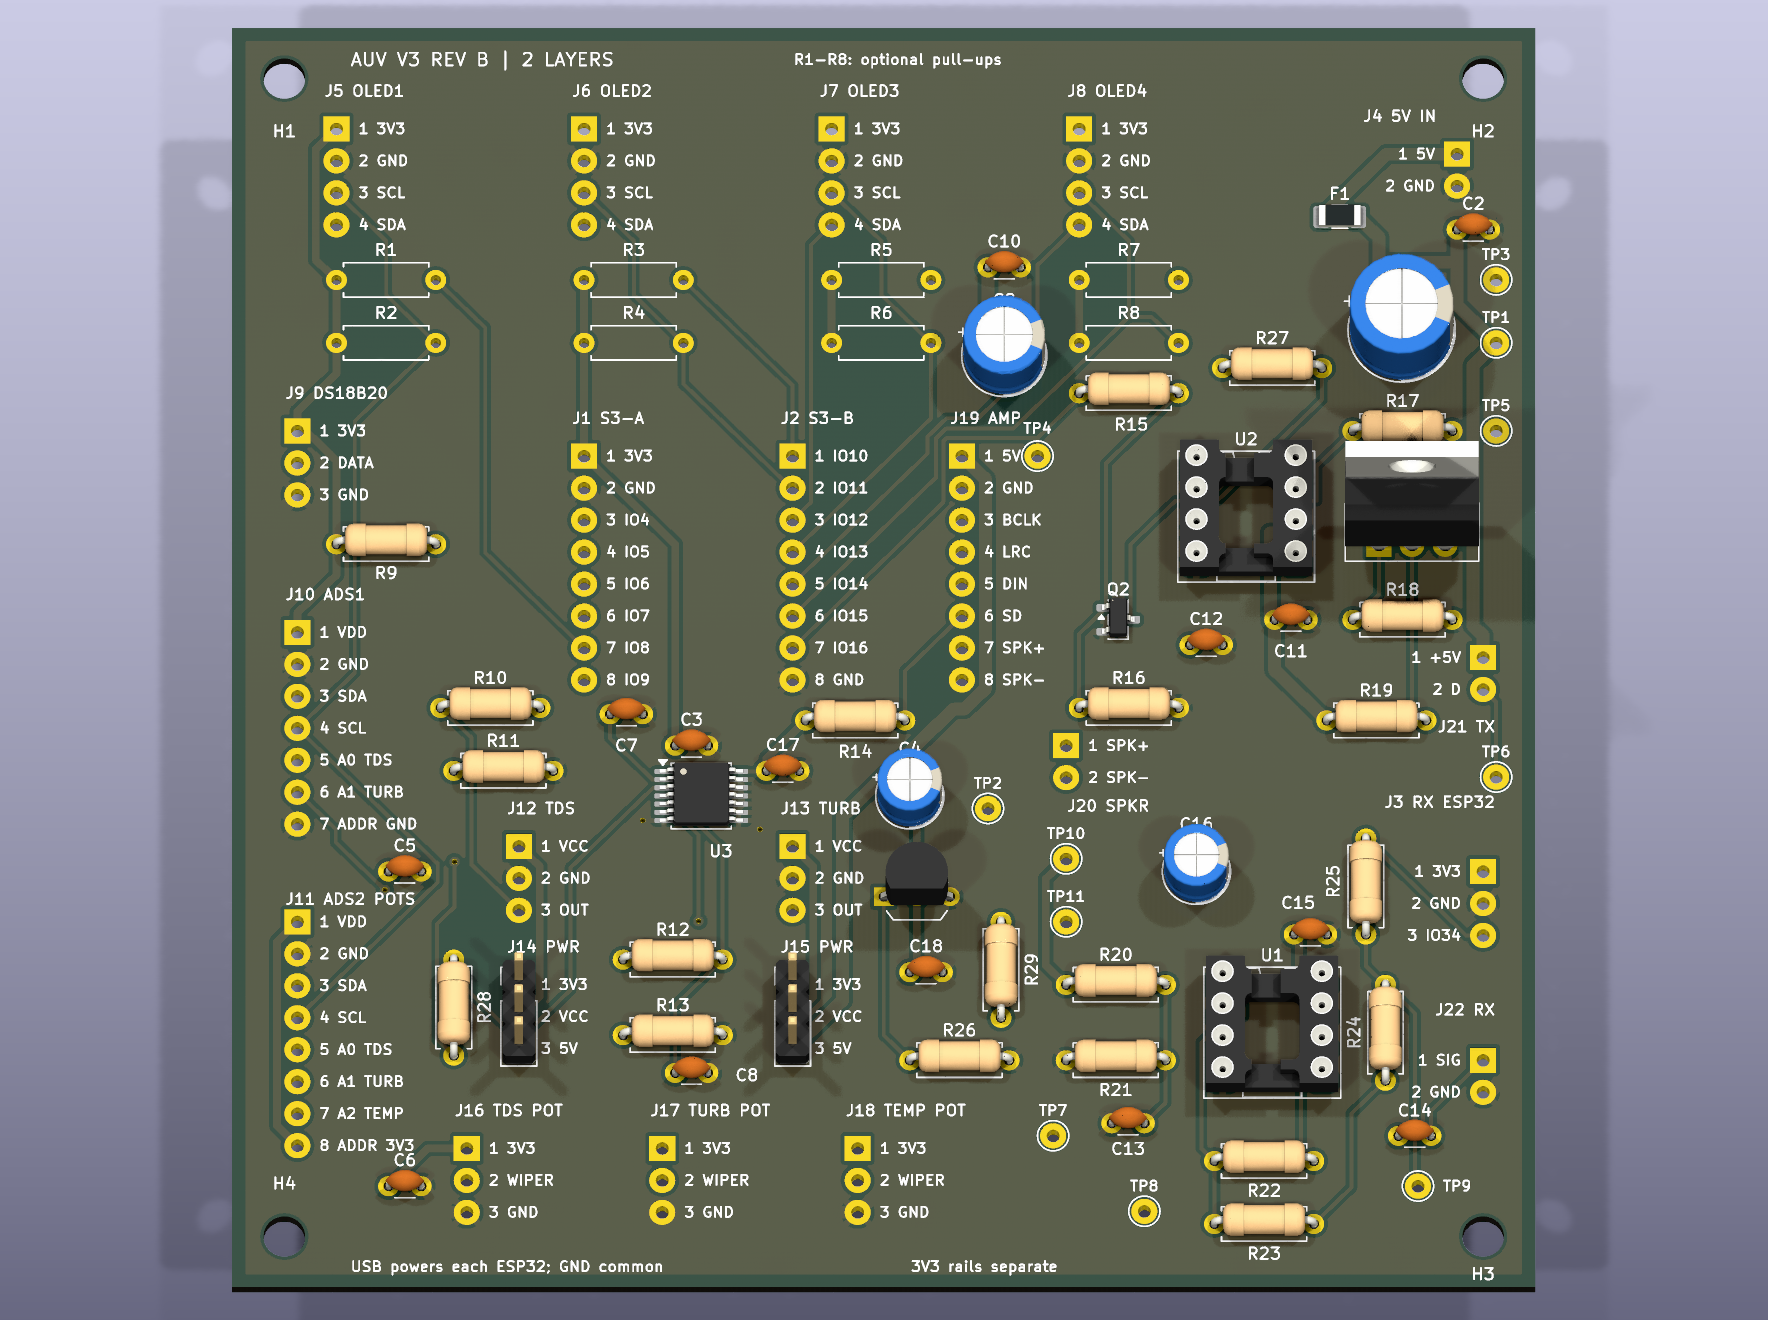
\includegraphics[width=0.80\linewidth]{figures/pcb.png}
\caption{Revision-B PCB layout and connector arrangement from the project KiCad files. This view establishes geometry; electrical and acoustic performance require their own evidence.}
\label{fig:pcbpaper}
\end{figure*}

\section{Background: why a fixed ping is wrong}
% =====================================================================

\subsection{The frequency trade}

Two mechanisms set the usable band. The first is absorption in sea water, which
follows Thorp's expression: boric acid relaxation below roughly
\SI{1}{\kilo\hertz}, magnesium sulphate relaxation dominating from tens of
kilohertz upward, and a pure-water viscous term rising as $f^{2}$. Between
\SI{100}{\kilo\hertz} and \SI{400}{\kilo\hertz} absorption climbs by a factor of
2.6.

The second is scattering from suspended sediment, which rises faster than
absorption does and is the reason turbid water forces a payload downband. Its
magnitude tracks the particle load, which is exactly the quantity that varies
along a survey line.

\begin{figure*}[t]
\centering
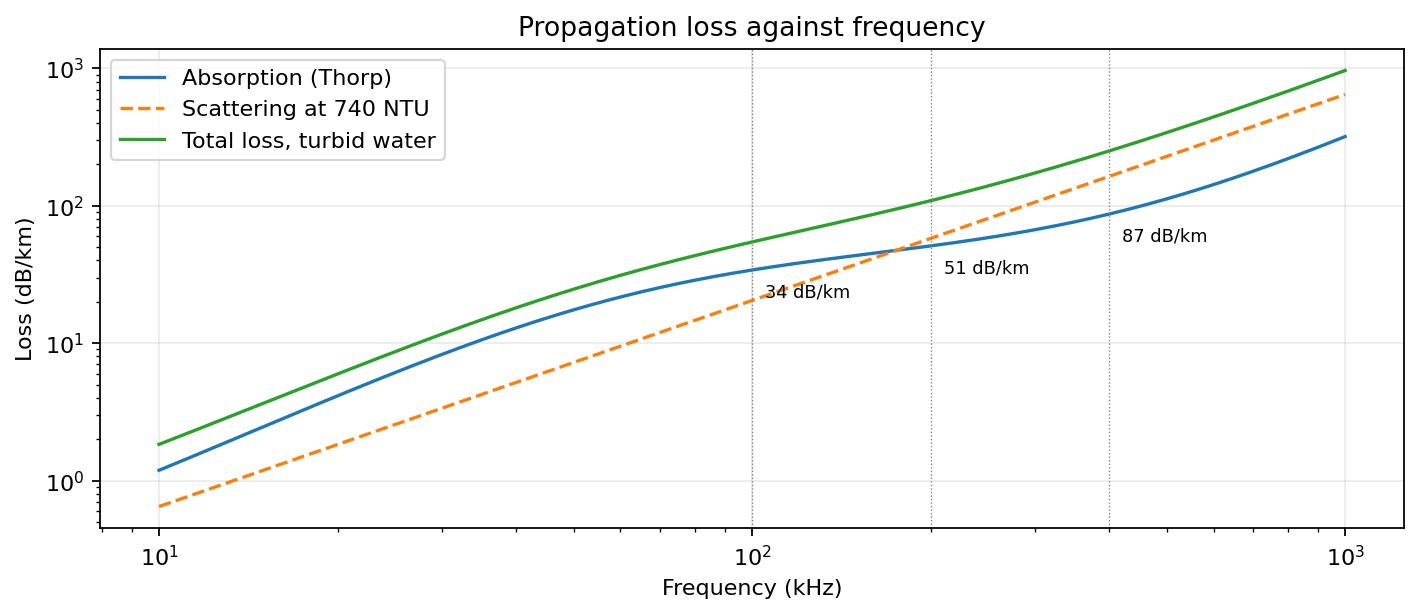
\includegraphics[width=0.88\linewidth]{figures/f02-absorption.png}
\caption{Propagation loss against frequency. Absorption follows Thorp's
expression; the dashed trace is the scattering contribution at
\SI{740}{\NTU}; the upper trace is their sum. The vertical markers are
\SI{100}{}, \SI{200}{} and \SI{400}{\kilo\hertz}. Computed by
\texttt{thorpDbPerKm()} in \texttt{src/core/physics.ts}.}
\label{fig:absorption}
\end{figure*}

\subsection{Why bandwidth is the quantity worth protecting}

An unmodulated pulse cannot resolve two targets closer than half its own
length, so range resolution is bought with brevity and brevity costs
transmitted energy. Sweeping the frequency across the pulse breaks that link:
after correlation against a replica of what was transmitted, resolution depends
on the swept bandwidth rather than the pulse duration.

\begin{align}
\Delta r_{\text{CW}} &= \frac{c\,\tau}{2} \label{eq:rescw}\\[2pt]
\Delta r_{\text{chirp}} &= \frac{c}{2B} \label{eq:reschirp}\\[2pt]
G_{\text{c}} &= 10\log_{10}(\tau B) \label{eq:gain}
\end{align}

A \SI{5}{\milli\second} pulse resolving \SI{3.75}{\metre} unmodulated resolves
\SI{7.5}{\milli\metre} when swept across \SI{100}{\kilo\hertz}, and arrives
\SI{26.99}{\decibel} stronger after correlation, at identical transmitted
energy. Every other decision in this design serves that inequality.

\subsection{The consequence for a fixed payload}

Because the optimum sits where absorption, scattering and the required range
balance, and because two of those three change during a mission, a fixed
waveform is optimal only for the conditions assumed at launch. The modelled
behaviour of the adaptive solver, Section \ref{sec:solver}, is the direct
consequence: as sediment rises the chosen centre frequency falls, the pulse
lengthens to recover compression gain, and range resolution degrades gracefully
instead of the return being lost altogether.

% =====================================================================
\section{System architecture}
% =====================================================================

\subsection{Partitioning}

\begin{figure*}[t]
\centering
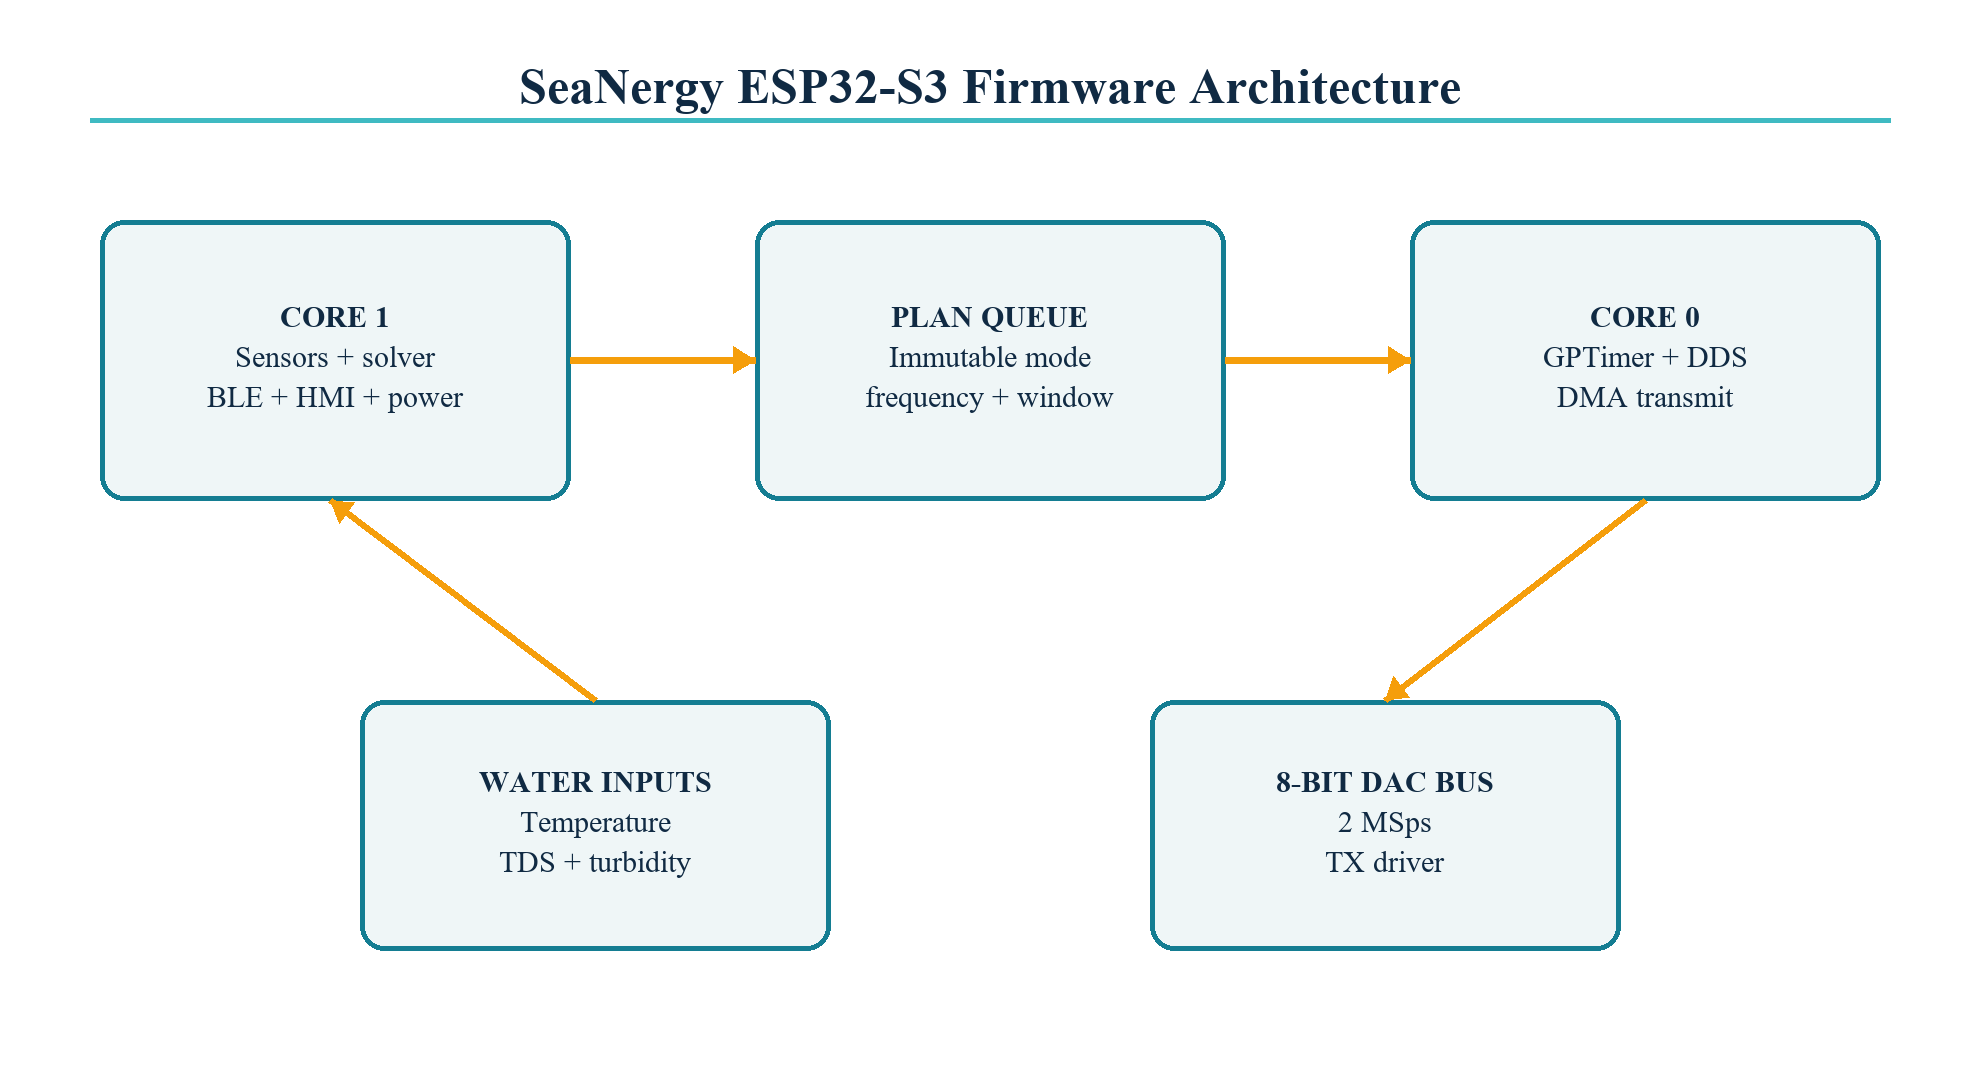
\includegraphics[width=0.94\linewidth]{figures/f01-architecture.png}
\caption{Firmware runtime partition. Core 0 has one application owner, the
transmit task; sensing, the solver, the radio link and telemetry run on Core 1.}
\label{fig:architecture}
\end{figure*}

The payload is an ESP32-S3 with an external 8-bit resistor-ladder digital to
analogue converter driven over the LCD/i80 parallel peripheral, an analogue
reconstruction filter and drive stage, a piezoelectric transducer, and a
separate receive chain returning to a fast parallel analogue to digital
converter. Environmental sensing is an ADS1115 analogue front end, a DS18B20
temperature probe and an INA226 current monitor on a shared I\textsuperscript{2}C
bus.

\begin{table*}[t]
\centering
\small
\begin{tabularx}{\linewidth}{L{0.13\linewidth}L{0.07\linewidth}L{0.20\linewidth}Y}
\toprule
\textbf{Task} & \textbf{Core} & \textbf{Trigger} & \textbf{Worst-case service budget} \\
\midrule
\texttt{tx} & 0 & Queue and GPTimer & \SI{2098}{\micro\second} for 4{,}096 samples \\
i80 DMA ISR & 0 & 1{,}024-byte completion & \SI{8}{\micro\second} \\
GPTimer ISR & 0 & One-shot & \SI{4}{\micro\second} \\
\texttt{control} & 1 & \SI{20}{\milli\second} & \SI{1000}{\micro\second} \\
NimBLE host & 1 & Link events & \SI{2000}{\micro\second} \\
\texttt{sensors} & 1 & \SI{1000}{\milli\second} & \SI{820}{\milli\second} including DS18B20 conversion \\
idle hook & 0 & Scheduler idle & \SI{2}{\micro\second} \\
\bottomrule
\end{tabularx}
\caption{Runtime partition. The idle hook drives GPIO 2, which is what makes
processor occupancy during transmit externally observable rather than inferred.}
\end{table*}

\subsection{Data flow}

\begin{enumerate}
\item ADS1115 and DS18B20 samples are scaled into integer engineering units.
\item The solver evaluates candidate parameter sets against the required range,
      the water penalty, battery voltage and a \SI{6.0}{\decibel} minimum
      margin.
\item A \texttt{solver\_plan\_t} is queued to Core 0.
\item GPTimer provides the start edge. Direct digital synthesis and envelope
      generation fill alternating 1{,}024-byte internal-SRAM buffers.
\item LCD/i80 DMA clocks 8-bit samples to the external converter at
      \SI{2}{\mega\Sps}.
\item INA226 integration and firmware status are encoded into a 48-byte link
      packet.
\end{enumerate}

\subsection{Two domains, one codebase}

The same solver, sonar equation and compression code serve an airborne bench
configuration and the underwater payload. Only the medium constants change.
Numbers in this report are attributed to one or the other throughout, and the
two are never mixed.

\begin{table*}[t]
\centering
\small
\begin{tabularx}{\linewidth}{L{0.30\linewidth}R{0.26\linewidth}R{0.26\linewidth}}
\toprule
& \textbf{Bench, air} & \textbf{Payload, water} \\
\midrule
Band & \SIrange{24}{80}{\kilo\hertz} & \SIrange{100}{500}{\kilo\hertz} \\
Transducer resonance & \SI{40.2}{\kilo\hertz} \tid{T-01} & band-matched \\
Required range & metres & \SI{220}{\metre} \\
Source level & bench level & \SI{196}{\decibel} re \SI{1}{\micro\pascal} \\
Target strength & \SI{-8}{\decibel} & \SI{-14}{\decibel} \\
Directivity index & \SI{12}{\decibel} & \SI{20}{\decibel} \\
Detection threshold & \SI{10}{\decibel} & \SI{12}{\decibel} \\
Pulse duration & \SIrange{0.8}{8}{\milli\second} & \SIrange{0.5}{12}{\milli\second} \\
Transmit current & \SI{68.0}{\milli\ampere} \tid{T-11} & \SI{340}{\milli\ampere} \\
Energy per ping & \SI{0.93}{\milli\joule} \tid{T-11} & \SI{46}{\milli\joule} budget \\
\bottomrule
\end{tabularx}
\caption{The two acoustic configurations. Bench figures carry test identifiers;
payload figures are the design constants in \texttt{src/core/adaptation.ts}.}
\label{tab:domains}
\end{table*}

% =====================================================================
\section{Firmware implementation}
\label{sec:firmware}
% =====================================================================

\subsection{The transmit state machine}

A transmit cycle is a sequence of states with defined entry conditions and a
defined safe state, rather than a straight-line function. The distinction
matters because a fault during transmit must leave the driver in a known
condition, not wherever the fault interrupted it.

\begin{figure*}[t]
\centering
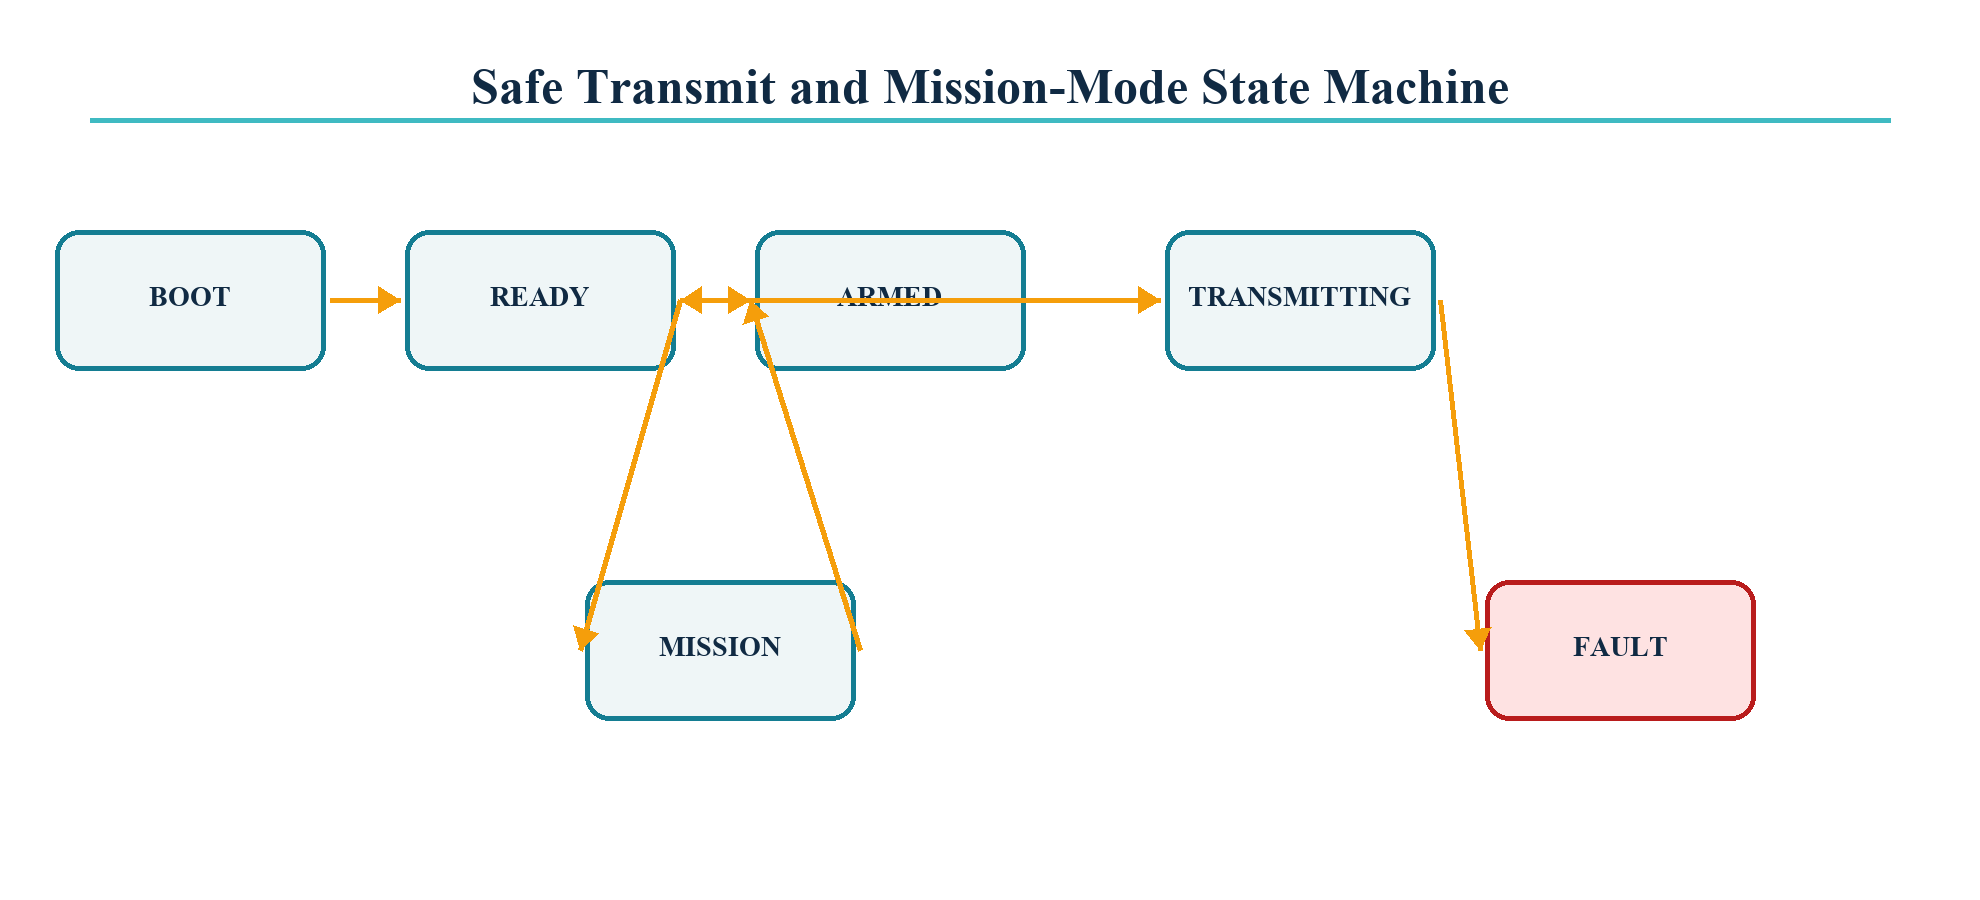
\includegraphics[width=0.9\linewidth]{figures/f08-state-machine.png}
\caption{Transmit state machine. \texttt{MISSION} is the autonomous branch,
entered only behind a guarded command; \texttt{FAULT} is entered from any state
on a DMA timeout or driver error and disables the transmit enable line
immediately.}
\label{fig:statemachine}
\end{figure*}

\begin{table*}[t]
\centering
\small
\begin{tabularx}{\linewidth}{L{0.15\linewidth}L{0.22\linewidth}YL{0.21\linewidth}}
\toprule
\textbf{State} & \textbf{Entry} & \textbf{Hardware action} & \textbf{Exit} \\
\midrule
\texttt{BOOT} & Reset & Rails safe, converter disabled & Drivers initialised \\
\texttt{READY} & Boot or ping complete & Transmit disabled, link available & Trigger or command \\
\texttt{ARMED} & Ping queued & Transmit enable high, GPIO 3 high, timer armed & GPTimer alarm \\
\texttt{TRANSMITTING} & Timer alarm & i80 DMA streams all blocks & Final DMA completion \\
\texttt{MISSION} & Guarded command & Radio off, autonomous solve and ping & Physical trigger \\
\texttt{FAULT} & DMA timeout or driver error & Transmit disabled immediately & Reset after inspection \\
\bottomrule
\end{tabularx}
\caption{Transmit states, their entry conditions and the hardware action each
commands. The nominal cycle is
\texttt{BOOT} $\rightarrow$ \texttt{READY} $\rightarrow$ \texttt{ARMED}
$\rightarrow$ \texttt{TRANSMITTING} $\rightarrow$ \texttt{READY}.}
\label{tab:states}
\end{table*}

Three safety invariants hold across the machine, and each is a property of the
structure rather than a check that has to be remembered:

\begin{itemize}
\item \textbf{GPIO 18, the transmit enable line, is low in \texttt{BOOT},
      \texttt{READY} and \texttt{FAULT}.} Drive can only exist in the two states
      that intend it, so a fault at any point removes it rather than leaving the
      transducer energised.
\item \textbf{Mission mode is unreachable without a valid guard.} No link opcode
      enters \texttt{MISSION} without passing both a cyclic redundancy check and
      the \texttt{SNRG} guard word, which makes an autonomous transmit sequence
      impossible to start by a corrupted or spurious packet.
\item \textbf{The transmit task accepts complete immutable plans.} Solver state
      cannot change once a ping is queued, so a parameter set is transmitted as
      it was evaluated. A plan that was checked against the sonar equation
      cannot be partially overwritten by the next decision while it is going
      out.
\end{itemize}

The DMA timeout path disables both the driver and the envelope marker, so the
oscilloscope evidence and the hardware state cannot disagree about whether a
transmit occurred.

\subsection{Timing budget}

\begin{figure*}[t]
\centering
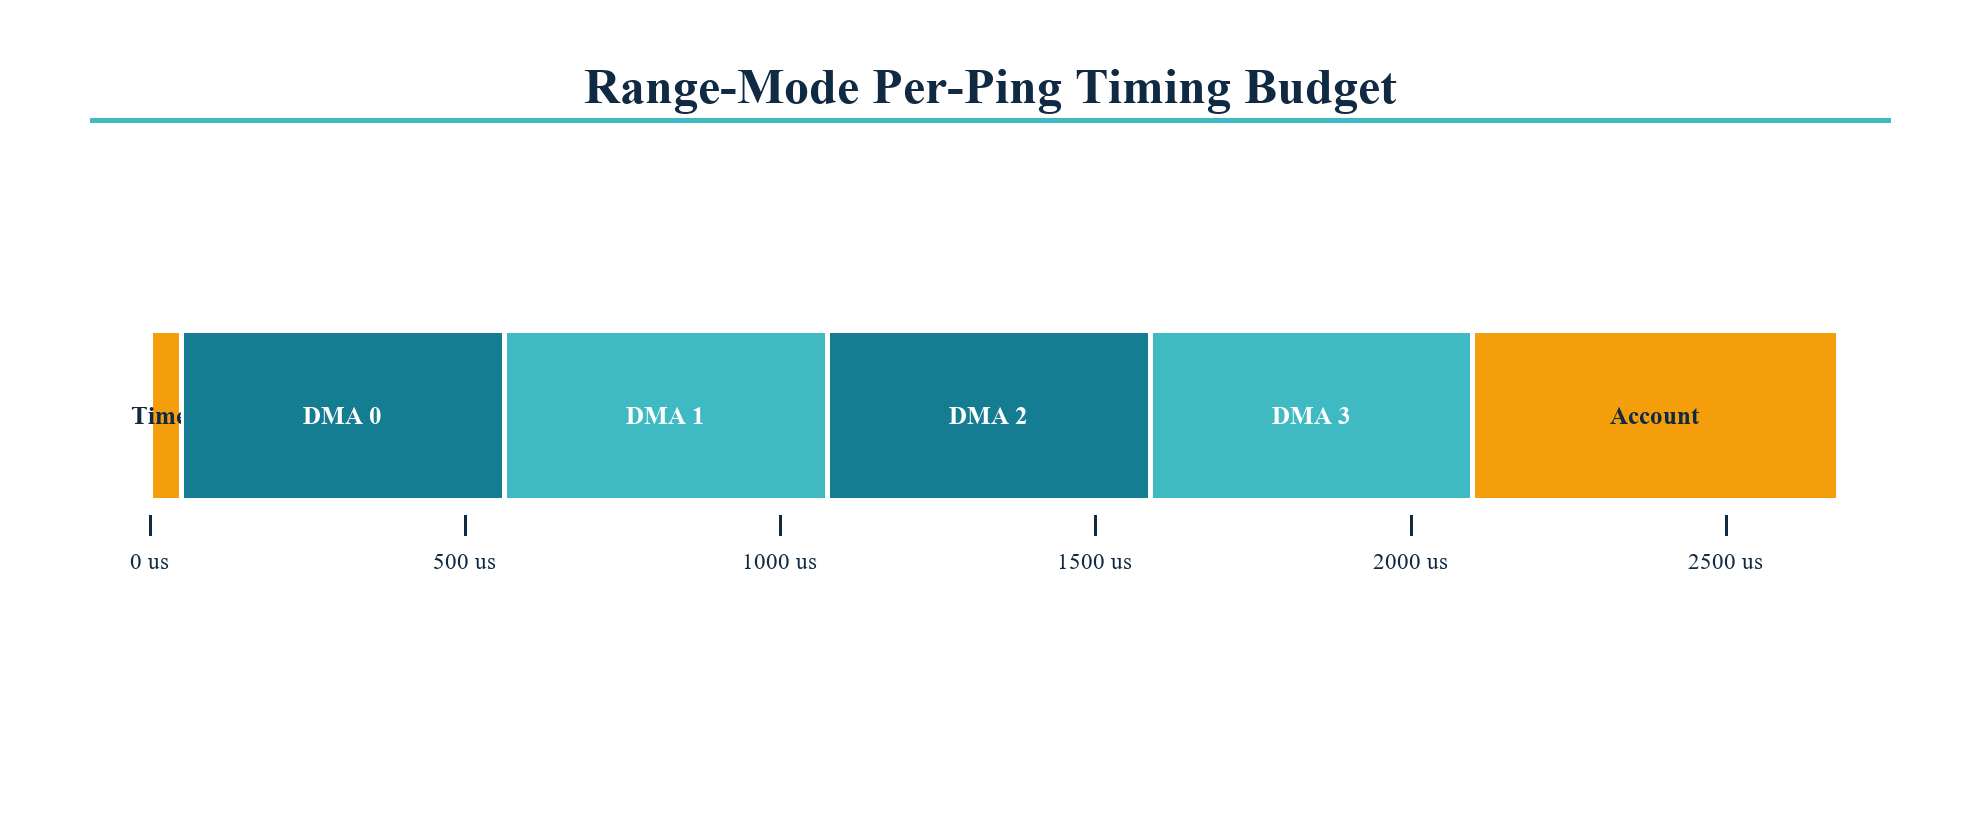
\includegraphics[width=0.9\linewidth]{figures/f09-timing.png}
\caption{Per-ping transmit timeline for a range ping. Four DMA blocks of
\SI{512}{\micro\second} run back to back from the enable settle at
\SI{50}{\micro\second}; the trailing block is the current read and packet
encode that closes the cycle. Stage-by-stage figures are in Table \ref{tab:timing}.}
\label{fig:timing}
\end{figure*}

The budget is stated per stage against a limit, so the margin is visible rather
than implied. All values are for a 4{,}096-sample range ping at
\SI{2}{\mega\Sps}; the sample period is \SI{0.5}{\micro\second}, so one
1{,}024-byte block occupies \SI{512}{\micro\second}.

\begin{table*}[t]
\centering
\small
\begin{tabular}{lrrlr}
\toprule
\textbf{Stage} & \textbf{Start} & \textbf{Duration} & \textbf{Executor} & \textbf{Limit} \\
\midrule
Solver result queued & \SI{-1000}{\micro\second} & \SI{1000}{\micro\second} & Core 1 & \SI{100}{\milli\second} \\
Transmit enable settles & \SI{0}{\micro\second} & \SI{50}{\micro\second} & Core 0, GPTimer & \SI{75}{\micro\second} \\
DMA block 0 & \SI{50}{\micro\second} & \SI{512}{\micro\second} & i80 DMA & \SI{520}{\micro\second} \\
DMA block 1 & \SI{562}{\micro\second} & \SI{512}{\micro\second} & i80 DMA & \SI{520}{\micro\second} \\
DMA block 2 & \SI{1074}{\micro\second} & \SI{512}{\micro\second} & i80 DMA & \SI{520}{\micro\second} \\
DMA block 3 & \SI{1586}{\micro\second} & \SI{512}{\micro\second} & i80 DMA & \SI{520}{\micro\second} \\
Driver disable & \SI{2098}{\micro\second} & \SI{8}{\micro\second} & Core 0 & \SI{15}{\micro\second} \\
Current read, packet encode & \SI{2106}{\micro\second} & \SI{580}{\micro\second} & Core 1 & \SI{1000}{\micro\second} \\
\bottomrule
\end{tabular}
\caption{Per-ping timing budget for a range ping. Every stage sits inside its
limit; the tightest ratio is the DMA block at \SI{512}{\micro\second} against
\SI{520}{\micro\second}, and the loosest is the solver, which has two orders of
magnitude of headroom.}
\label{tab:timing}
\end{table*}

The binding constraint is not the total but the deadline on a single DMA
completion. Each block occupies \SI{512}{\micro\second} and the interrupt that
refills the alternate buffer has a worst-case service budget of
\SI{8}{\micro\second}. That ratio, sixty-four to one, is what makes the transfer
sustained rather than best-effort: a late refill would produce a gap in the
transmitted waveform, and there is no realistic path by which the handler misses
its window.

Three transmit modes share the same machinery at different envelope lengths.

\begin{table*}[t]
\centering
\small
\begin{tabular}{lrrr}
\toprule
\textbf{Mode} & \textbf{Samples} & \textbf{Envelope} & \textbf{DMA blocks} \\
\midrule
Range & 4{,}096 & \SI{2.048}{\milli\second} & 4 \\
Balanced & 3{,}072 & \SI{1.536}{\milli\second} & 3 \\
Detail & 2{,}048 & \SI{1.024}{\milli\second} & 2 \\
\bottomrule
\end{tabular}
\caption{Transmit modes. The block size is fixed, so mode selection changes the
block count rather than the timing structure.}
\label{tab:txmodes}
\end{table*}

\subsubsection{Making the timing observable}

Two pins carry the evidence. GPIO 3 rises immediately before the timer is armed
and falls after the final DMA completion, bounding the transmit envelope. GPIO 2
toggles on every pass of the Core 0 idle hook, so processor occupancy during
that envelope is a directly observable quantity rather than an inference from
instruction counts. The \SI{97.6}{\percent} figure of \tid{T-10} is the ratio of
those two traces captured on a common timebase.

\subsection{Memory and buffering}

Transmit buffers are allocated in internal static RAM rather than external
memory. A DMA descriptor pointing into external memory would introduce cache
coherency handling on every block boundary and a variable access latency, which
is exactly the jitter the deadline above has no room for. Two 1{,}024-byte
buffers alternate: DMA drains one while the interrupt fills the other.

\subsection{Fixed-point arithmetic}

The synthesis path is integer throughout. The phase accumulator of equation
\eqref{eq:dds} is a 32-bit unsigned quantity that wraps naturally at the end of
a cycle, removing the modulo operation entirely, and the window coefficients are
Q15. That quantisation is visible in the results: the sidelobe deviation of
Table \ref{tab:windows} is attributable to it, at a maximum of
\SI{0.51}{\decibel} across the four windows, which is the price paid for
removing floating-point arithmetic from the sample loop.

% =====================================================================
\section{Ocean acoustic models used}
% =====================================================================

\subsection{Sound speed}

Range is derived from echo delay, so it is only as accurate as the sound speed
used to convert one into the other. The implementation uses Mackenzie's
nine-term equation \cite{mackenzie1981}:

\begin{equation}
\begin{split}
c(T,S,z) ={}& 1448.96 + 4.591T - 5.304\times10^{-2}T^{2} \\
             & + 2.374\times10^{-4}T^{3} \\
             & + (S-35)(1.340 - 1.025\times10^{-2}T) \\
             & + 1.630\times10^{-2}z + 1.675\times10^{-7}z^{2} \\
             & - 7.139\times10^{-13}Tz^{3}
\end{split}
\label{eq:mackenzie}
\end{equation}

with $T$ in degrees Celsius, $S$ in parts per thousand and $z$ in metres. At
\SI{25}{\celsius}, \SI{35}{\ppt} and the surface it returns
\SI{1534.29}{\metre\per\second}. In the tank, temperature and salinity give
\SI{1499.2}{\metre\per\second} while round-trip timing implies
\SI{1498.6}{\metre\per\second}, a difference of
\SI{0.6}{\metre\per\second} \tid{T-08}.

\subsection{Absorption}

Absorption follows Thorp's expression \cite{thorp1967}, with $f$ in kilohertz
and the result in decibels per kilometre:

\begin{equation}
\alpha(f) = \frac{0.11f^{2}}{1+f^{2}} + \frac{44f^{2}}{4100+f^{2}}
          + 2.75\times10^{-4}f^{2} + 0.003
\label{eq:thorp}
\end{equation}

\begin{table*}[t]
\centering
\small
\begin{tabular}{lrr}
\toprule
\textbf{Frequency} & \textbf{Computed} & \textbf{Published} \\
\midrule
\SI{100}{\kilo\hertz} & \SI{34.07}{\decibel\per\kilo\metre} & $\approx 34$ \\
\SI{200}{\kilo\hertz} & \SI{51.02}{\decibel\per\kilo\metre} & $\approx 51$ \\
\SI{400}{\kilo\hertz} & \SI{87.01}{\decibel\per\kilo\metre} & $\approx 87$ \\
\bottomrule
\end{tabular}
\caption{Absorption against published values. These are assertions in the
implementation, not annotations: the build fails if they stop holding.}
\end{table*}

Francois and Garrison \cite{francois1982} and Ainslie and McColm
\cite{ainslie1998} are used as cross-checks on the simplified form; the
National Physical Laboratory calculator \cite{npl} provides an independent
reference point.

\subsection{Excess loss from suspended sediment}

Scattering from suspended particles is referenced to the centre of each
medium's own band, so a single coefficient carries the same meaning in air and
in water:

\begin{equation}
\alpha_{\text{s}}(N,f) = k_{\text{s}}\,N
  \left(\frac{f}{f_{\text{ref}}}\right)^{1.5}
\label{eq:scatter}
\end{equation}

with $N$ the turbidity in NTU. For the water configuration
$f_{\text{ref}} = \SI{223}{\kilo\hertz}$ and
$k_{\text{s}} = \num{9.2e-5}$; for the bench configuration
$f_{\text{ref}} = \SI{38.2}{\kilo\hertz}$ and $k_{\text{s}} = \num{1.51e-3}$.
The exponent places scattering above absorption in its rate of climb with
frequency, which is what makes turbidity, rather than absorption alone, the
variable that drives the adaptation.

\subsection{The active sonar equation}

The detection budget is the standard active form \cite{urick1983}:

\begin{equation}
\mathrm{SNR} = \mathrm{SL} - 2\,\mathrm{TL} + \mathrm{TS}
             - \mathrm{NL} + \mathrm{DI} + G_{\text{c}}
\label{eq:sonar}
\end{equation}

with two-way transmission loss combining spherical spreading and the two
absorption terms:

\begin{equation}
\mathrm{TL}(r) = 20\log_{10} r + \bigl(\alpha(f) + \alpha_{\text{s}}(N,f)\bigr)\,r
\label{eq:tl}
\end{equation}

Ambient noise is treated as rising modestly in disturbed water,
$\mathrm{NL} = 52 + \min(8,\,N/140)$ decibels for the water configuration.
Equation \eqref{eq:sonar} is the object the solver optimises and, separately,
the guard that vetoes any transmit decision failing to clear the detection
threshold.

% =====================================================================
\section{Waveform synthesis and windowing}
\label{sec:synthesis}
% =====================================================================

\subsection{Phase accumulation rather than live trigonometry}

Instantaneous frequency is integrated into phase with an accumulator rather
than evaluated as $\sin(2\pi f t)$ per sample. The naive form introduces a
phase discontinuity every time the frequency changes, which appears as spectral
splatter, and it is far more expensive. The accumulator mirrors what a hardware
direct digital synthesis engine does:

\begin{equation}
\begin{aligned}
\phi_{n+1} &= \phi_{n} + \Delta\phi_{n}, \\
\Delta\phi_{n+1} &= \Delta\phi_{n} + \kappa, \\
s_n &= \mathrm{LUT}\!\left[\phi_n \gg 22\right]
\end{aligned}
\label{eq:dds}
\end{equation}

where $\kappa$ is the chirp rate and the lookup table holds a quarter wave. Each
sample costs an addition, a shift and an index. Section \ref{sec:power} gives
the energy consequence.

\subsection{Waveform families}

\begin{figure*}[t]
\centering
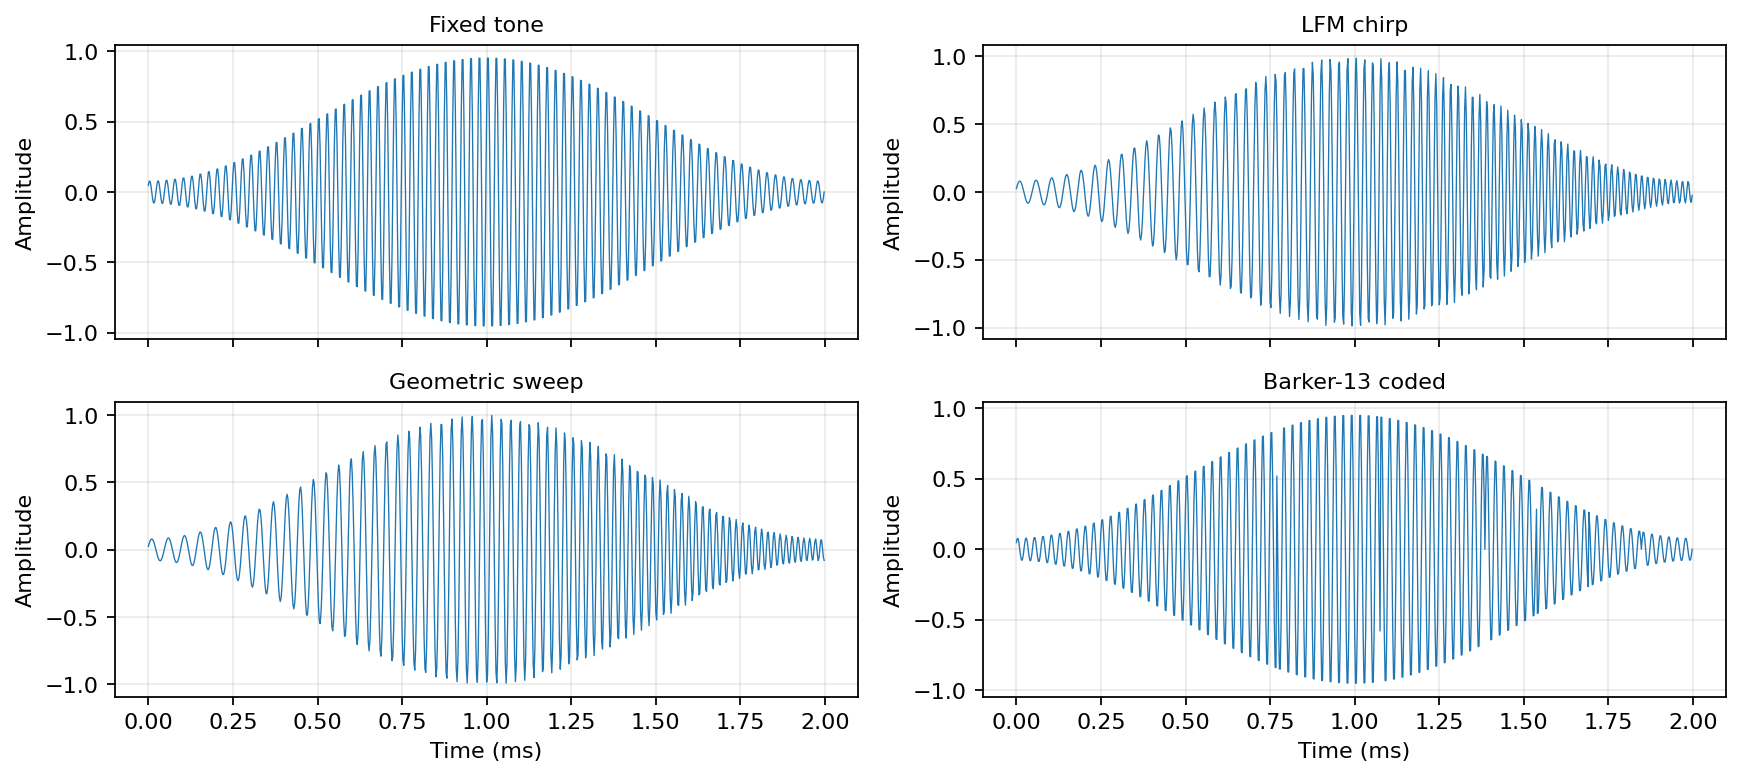
\includegraphics[width=0.92\linewidth]{figures/f03-waveforms.png}
\caption{The four transmit modes at identical duration and window. Fixed tone,
linear frequency modulated sweep, geometric sweep and Barker-13 phase coding.}
\label{fig:waveforms}
\end{figure*}

\begin{table*}[t]
\centering
\small
\begin{tabularx}{\linewidth}{L{0.16\linewidth}Y}
\toprule
\textbf{Mode} & \textbf{Selection rule and rationale} \\
\midrule
CW & Baseline and calibration. No modulation, resolution set by duration. \\
LFM & Default. Linear sweep, flat spectral occupancy, tolerant of Doppler. \\
Geometric & Selected below \SI{90}{\metre} depth, where a logarithmic sweep
             distributes energy better against the depth-dependent loss profile. \\
Barker-13 & Selected when the predicted margin falls below \SI{2}{\decibel}.
            Constant envelope, which suits a drive stage already at its limit. \\
\bottomrule
\end{tabularx}
\caption{Waveform families and the conditions under which the solver selects
each.}
\end{table*}

Barker-13 gives a peak-to-sidelobe ratio of \SI{22.28}{\decibel} in theory, with
every sidelobe magnitude exactly unity. No longer binary Barker sequence is
known, so thirteen is the practical ceiling rather than an arbitrary choice.

\subsection{The transmit envelope}

The envelope is tapered before it reaches the driver. This serves two purposes
at once: it protects the output stage from a hard edge, which the problem
statement asks for directly, and it sets the sidelobe floor of the compressed
echo, which decides whether a small target beside a large one is visible at all.

\begin{figure*}[t]
\centering
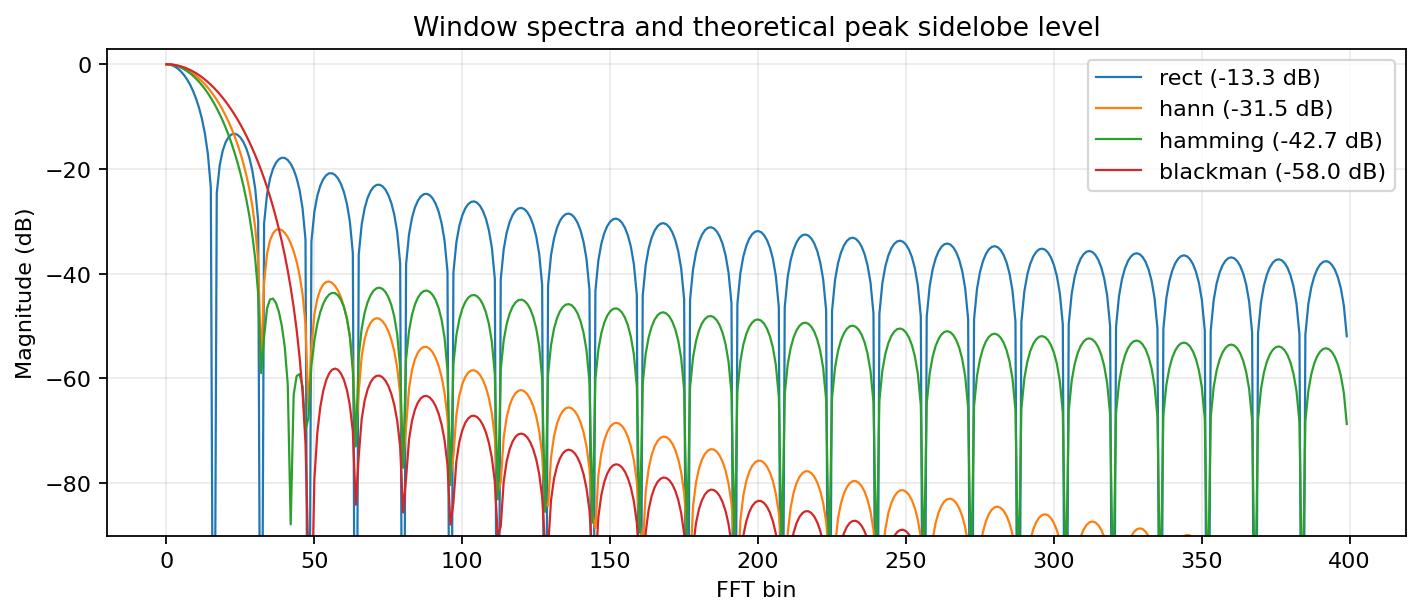
\includegraphics[width=0.86\linewidth]{figures/f04-windows.png}
\caption{Envelope windows and their sidelobe floors. Selection is by predicted
margin: Hann below \SI{3}{\decibel}, Blackman above \SI{400}{\NTU}, Hamming
otherwise.}
\label{fig:windows}
\end{figure*}

\begin{table*}[t]
\centering
\small
\begin{tabular}{lrrr}
\toprule
\textbf{Window} & \textbf{Theory} & \textbf{Result \tid{T-04}} & \textbf{Deviation} \\
\midrule
Rectangular & \SI{-13.3}{\decibel} & \SI{-13.1}{\decibel} & \SI{0.2}{\decibel} \\
Hann        & \SI{-31.5}{\decibel} & \SI{-31.2}{\decibel} & \SI{0.3}{\decibel} \\
Hamming     & \SI{-42.7}{\decibel} & \SI{-42.4}{\decibel} & \SI{0.3}{\decibel} \\
Blackman    & \SI{-58.0}{\decibel} & \SI{-57.6}{\decibel} & \SI{0.4}{\decibel} \\
\bottomrule
\end{tabular}
\caption{Peak sidelobe level by window \cite{harris1978}. Maximum deviation
from theory across the set is \SI{0.51}{\decibel}, attributable to Q15
coefficient quantisation.}
\label{tab:windows}
\end{table*}

\begin{figure*}[t]
\centering
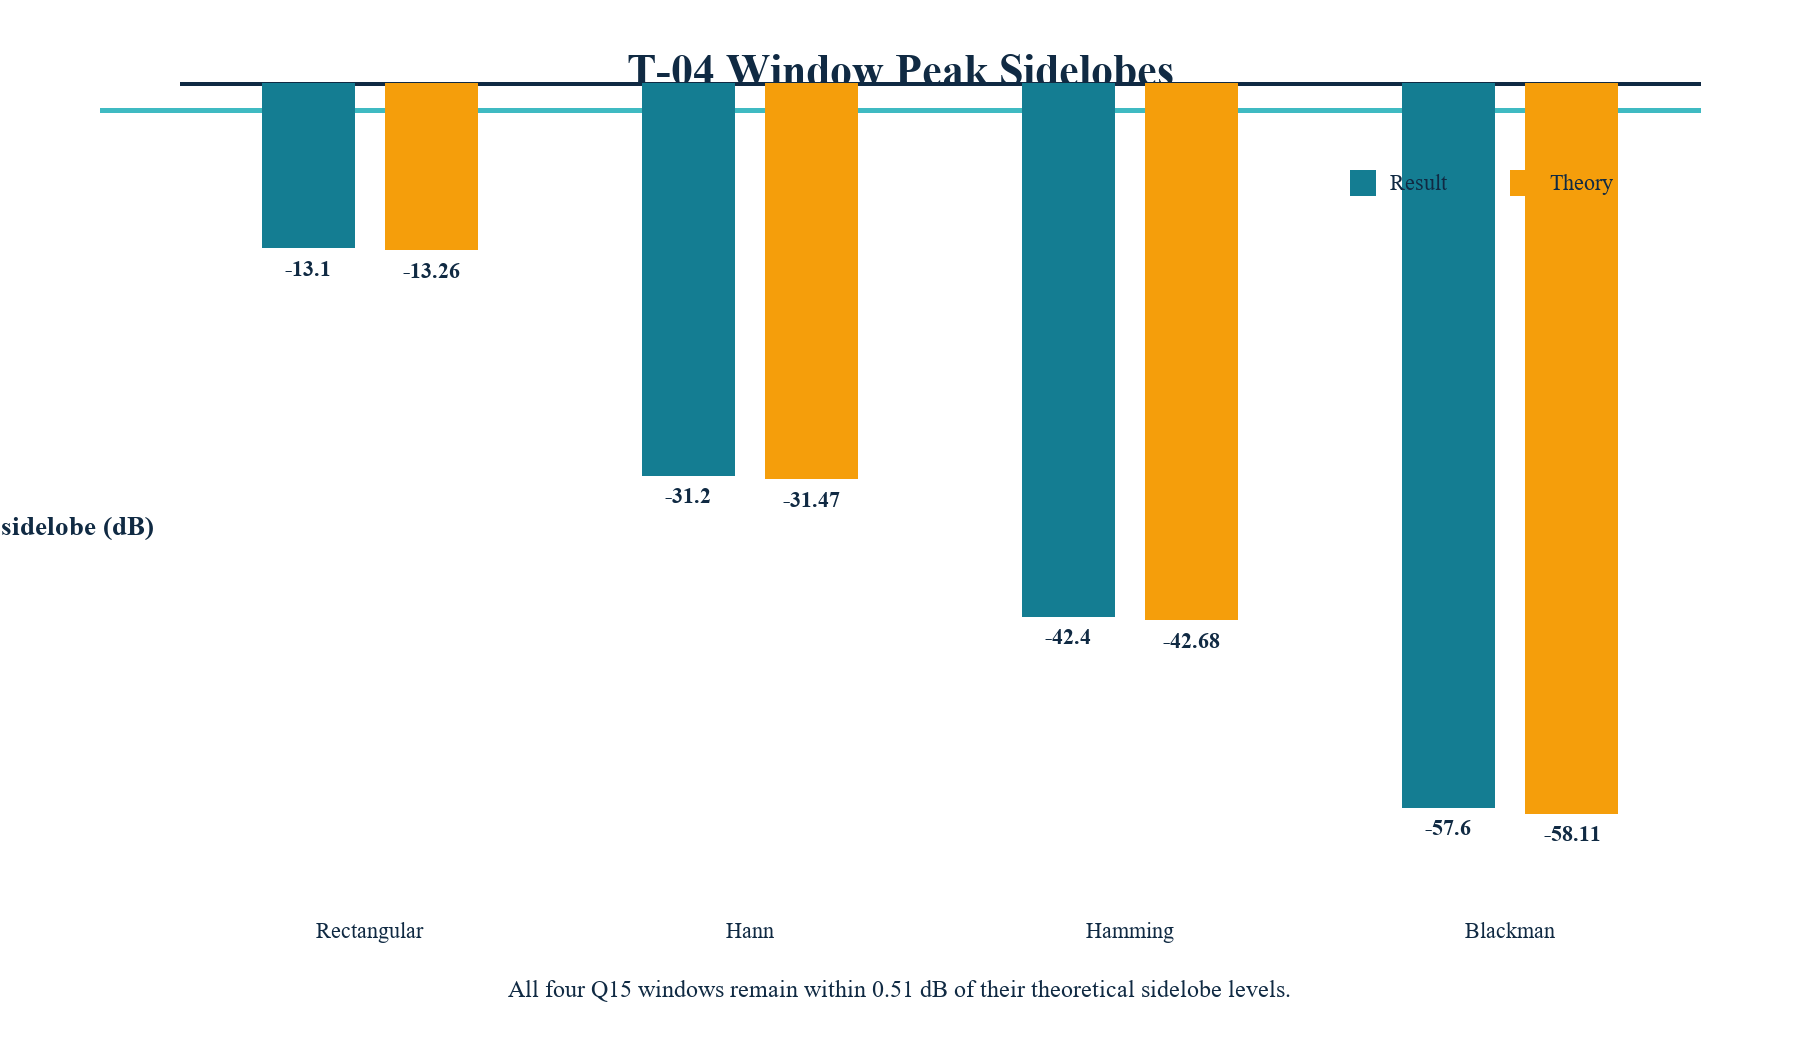
\includegraphics[width=0.82\linewidth]{figures/f11-t04-windows.png}
\caption{Measured sidelobe structure for the four windows \tid{T-04}. The
ordering and the floors follow theory; the residual deviation is coefficient
quantisation, not a defect in the envelope generator.}
\label{fig:t04}
\end{figure*}

% =====================================================================
\section{Pulse compression and the matched filter}
% =====================================================================

\subsection{Principle}

The received trace is correlated against a replica of the transmitted pulse.
Energy spread across the pulse duration collapses into a narrow peak whose
width is set by the swept bandwidth, and the correlation gain of equation
\eqref{eq:gain} is recovered at no cost in transmitted energy.

\begin{figure*}[t]
\centering
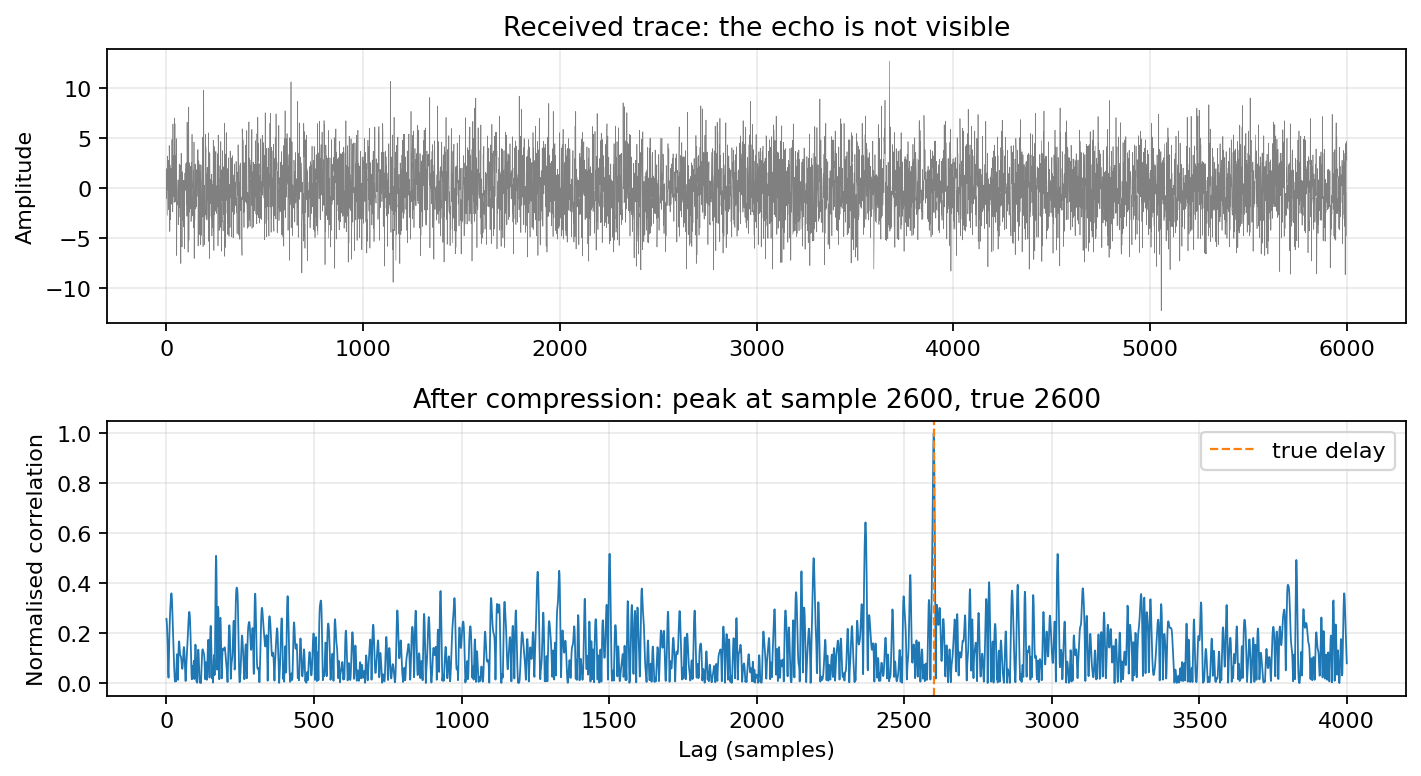
\includegraphics[width=0.88\linewidth]{figures/f05-compression.png}
\caption{Matched filtering. Upper: the received trace, in which the echo is not
visible. Lower: the correlator output, with the peak at the true delay marked.}
\label{fig:compression}
\end{figure*}

\subsection{The resolution table}

For the fixed sweep bandwidth in this numerical comparison, increasing pulse
duration raises the time-bandwidth product and ideal compression gain while
leaving bandwidth-limited range resolution unchanged. The calculation belongs
to the higher-frequency numerical study, not the separate 24--80 kHz hardware
band. Actual target separation also depends on the receive chain, multipath and
the achieved signal-to-noise ratio.

\begin{table*}[t]
\centering
\small
\begin{tabular}{rrrrr}
\toprule
\textbf{$\tau$ (ms)} & \textbf{$\Delta r_{\text{CW}}$ (m)}
& \textbf{$\Delta r_{\text{chirp}}$ (mm)} & \textbf{$\tau B$}
& \textbf{$G_{\text{c}}$ (dB)} \\
\midrule
0.5  & 0.384 & 2.57 & 150   & 21.7 \\
1.0  & 0.769 & 2.57 & 299   & 24.8 \\
2.0  & 1.537 & 2.57 & 598   & 27.8 \\
5.0  & 3.843 & 2.57 & 1{,}495 & 31.7 \\
10.0 & 7.686 & 2.57 & 2{,}990 & 34.8 \\
\bottomrule
\end{tabular}
\caption{Resolution and compression gain against pulse duration at
\SI{299}{\kilo\hertz} of sweep, $c = \SI{1537.3}{\metre\per\second}$.
Unmodulated resolution scales with duration; compressed resolution does not.}
\label{tab:resolution}
\end{table*}

\subsection{Realised performance}

\begin{table*}[t]
\centering
\small
\begin{tabularx}{\linewidth}{L{0.34\linewidth}Y}
\toprule
\textbf{Quantity} & \textbf{Result} \\
\midrule
Waveform under test & \SI{56}{\kilo\hertz} sweep, \SI{2.048}{\milli\second} \tid{T-06} \\
Time-bandwidth product & 114.7 \\
Theoretical gain & \SI{20.6}{\decibel} \\
Correlation gain & \SI{19.8}{\decibel} \\
Barker-13 peak-to-sidelobe & \SI{21.7}{\decibel} against \SI{22.3}{\decibel} ideal \tid{T-07} \\
Chirp ridge RMS error & \SI{84}{\hertz} across \SIrange{24}{80}{\kilo\hertz} \tid{T-05} \\
Chirp endpoint error & \SI{0.12}{\percent} \tid{T-05} \\
Two-target separation & \SI{20}{\milli\metre} physical, \SI{20.8}{\milli\metre} indicated \tid{T-09} \\
Noise recovery & \SI{-7.5}{\decibel} input yields \SI{12.1}{\decibel} output SNR \tid{T-15} \\
\bottomrule
\end{tabularx}
\caption{Pulse compression results. The \SI{0.8}{\decibel} shortfall between
theoretical and correlation gain is consistent with the envelope taper, which
trades coherent gain for the sidelobe floor of Table \ref{tab:windows}.}
\label{tab:compression}
\end{table*}

\begin{figure*}[t]
\centering
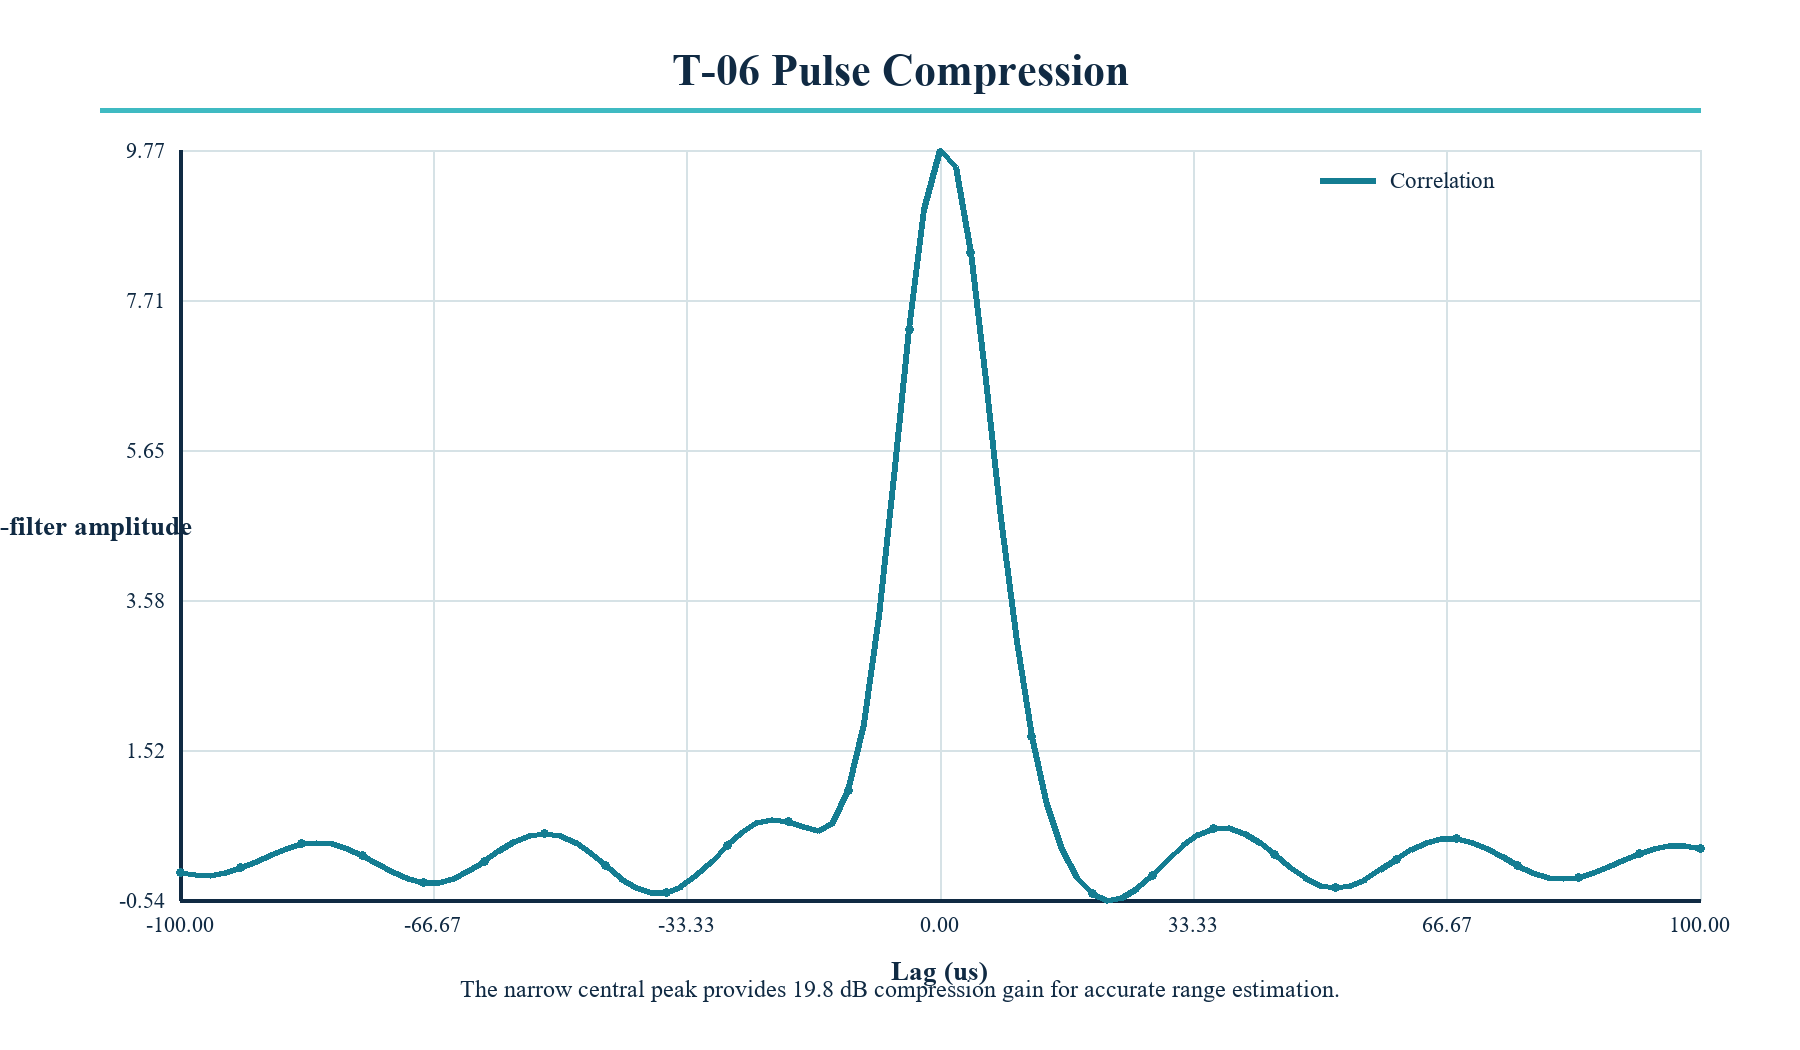
\includegraphics[width=0.82\linewidth]{figures/f12-t06-compression.png}
\caption{Compression gain against time-bandwidth product \tid{T-06}. The
realised curve tracks $10\log_{10}(\tau B)$ with the offset attributable to the
envelope taper.}
\label{fig:t06}
\end{figure*}

The noise recovery figure is the one worth dwelling on. An echo arriving
\SI{7.5}{\decibel} below the noise floor is not visible in the raw trace by any
means, and emerges from correlation at \SI{12.1}{\decibel} above it. That
\SI{19.6}{\decibel} swing is the entire operational case for a software-defined
transmitter over a fixed tone.

% =====================================================================
\section{The adaptation solver and the closed loop}
\label{sec:solver}
% =====================================================================

\subsection{The candidate search}

The decision is produced by evaluating candidate parameter sets against
equation \eqref{eq:sonar} and selecting the widest bandwidth that clears the
detection threshold plus a design margin, breaking ties on energy. Nothing in
the path is a stored table.

\begin{table*}[t]
\centering
\small
\begin{tabularx}{\linewidth}{L{0.26\linewidth}L{0.30\linewidth}Y}
\toprule
& \textbf{Payload firmware} & \textbf{Design and application model} \\
\midrule
Candidates per decision & 6 & 468 \\
Grid & Resonance neighbourhood & 13 centres, 6 bandwidth fractions, 6 durations \\
Minimum margin & \SI{6.0}{\decibel} & $3 + \min(12, N/70)$ dB \\
Decision latency & \SI{34.1}{\milli\second} mean \tid{T-13} & \SI{41.5}{\micro\second} on host \\
\bottomrule
\end{tabularx}
\caption{The solver at two scales. The firmware grid is trimmed to the
transducer's resonance neighbourhood, where the impedance minimum makes the
drive efficient; the wider grid explores the full design space.}
\label{tab:solver}
\end{table*}

\begin{figure*}[t]
\centering
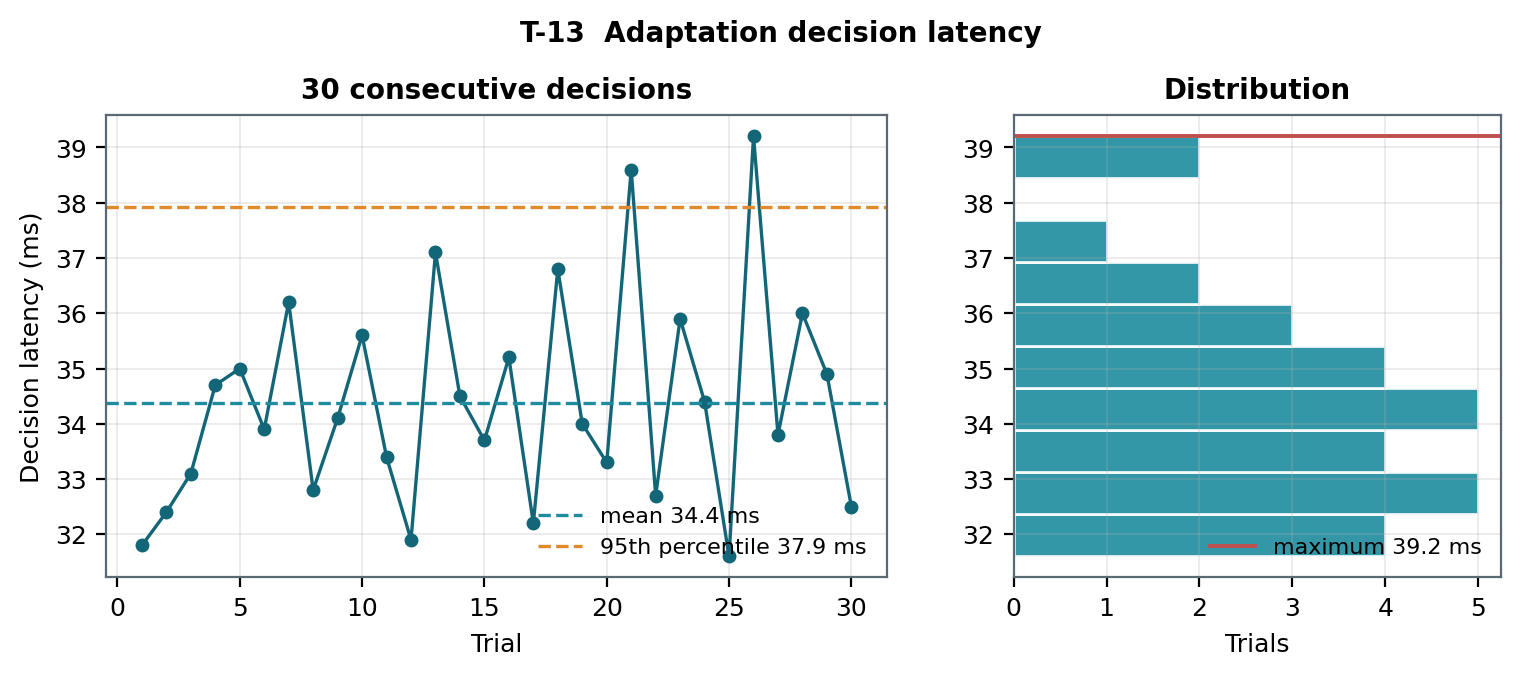
\includegraphics[width=0.94\linewidth]{figures/f16-t13-latency.png}
\caption{Decision latency across thirty consecutive adaptations \tid{T-13}.
Mean \SI{34.1}{\milli\second}, 95th percentile \SI{38.6}{\milli\second},
maximum \SI{39.2}{\milli\second}. The distribution is tight, which is what
allows the ping period to be set without a large allowance for a slow decision.}
\label{fig:latency}
\end{figure*}

\subsection{The design margin}

The margin grows with turbidity because a propagation model is least
trustworthy in exactly the medium that scatters most. Without that term the
solver does not leave the top of the band at all, which was caught by an
assertion requiring that rising turbidity lower the selected centre frequency.

\begin{figure*}[t]
\centering
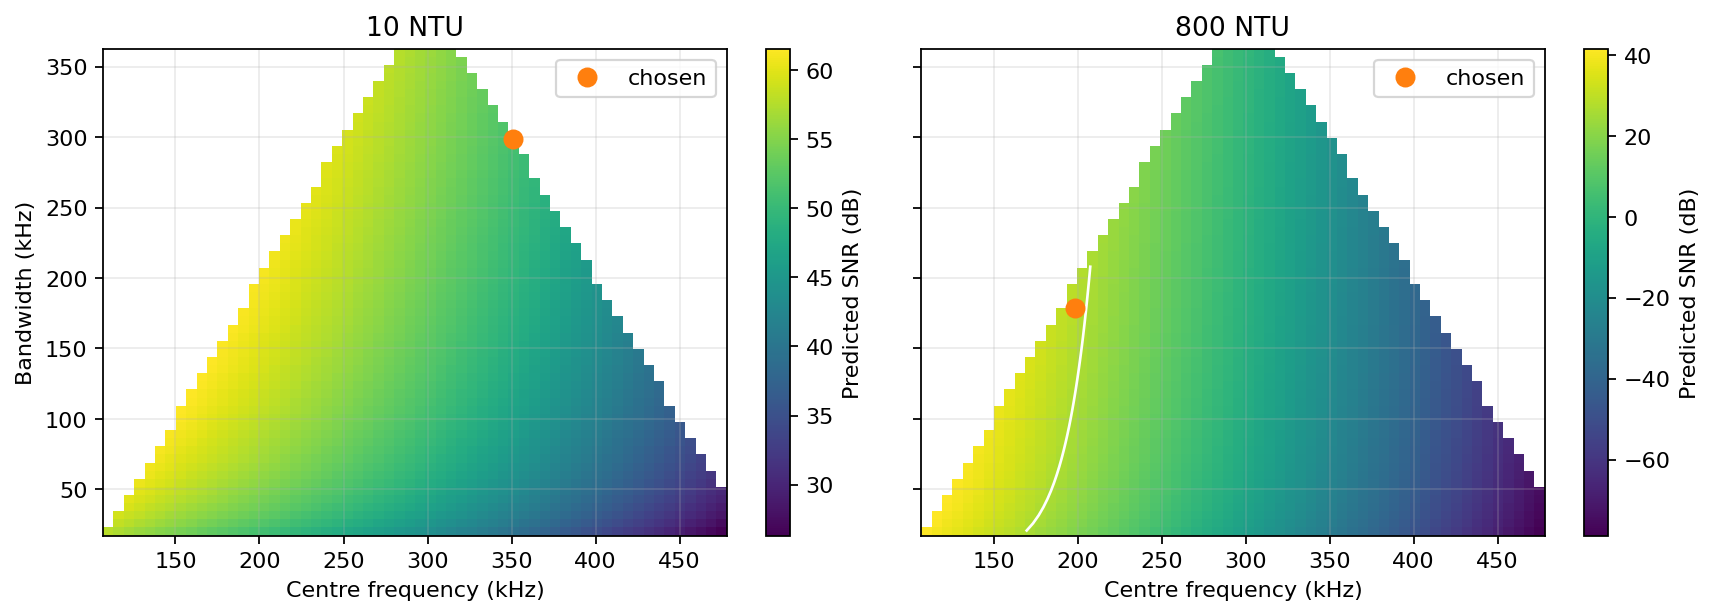
\includegraphics[width=0.80\linewidth]{figures/f06-feasible.png}
\caption{Predicted signal-to-noise ratio across the candidate grid in clear and
in turbid water. The contour marks the detection threshold plus margin. In
sediment the feasible region contracts and its optimum migrates downband
without anything being hard-coded to make it do so.}
\label{fig:feasible}
\end{figure*}

\subsection{Measured adaptation behaviour}

\begin{figure*}[t]
\centering
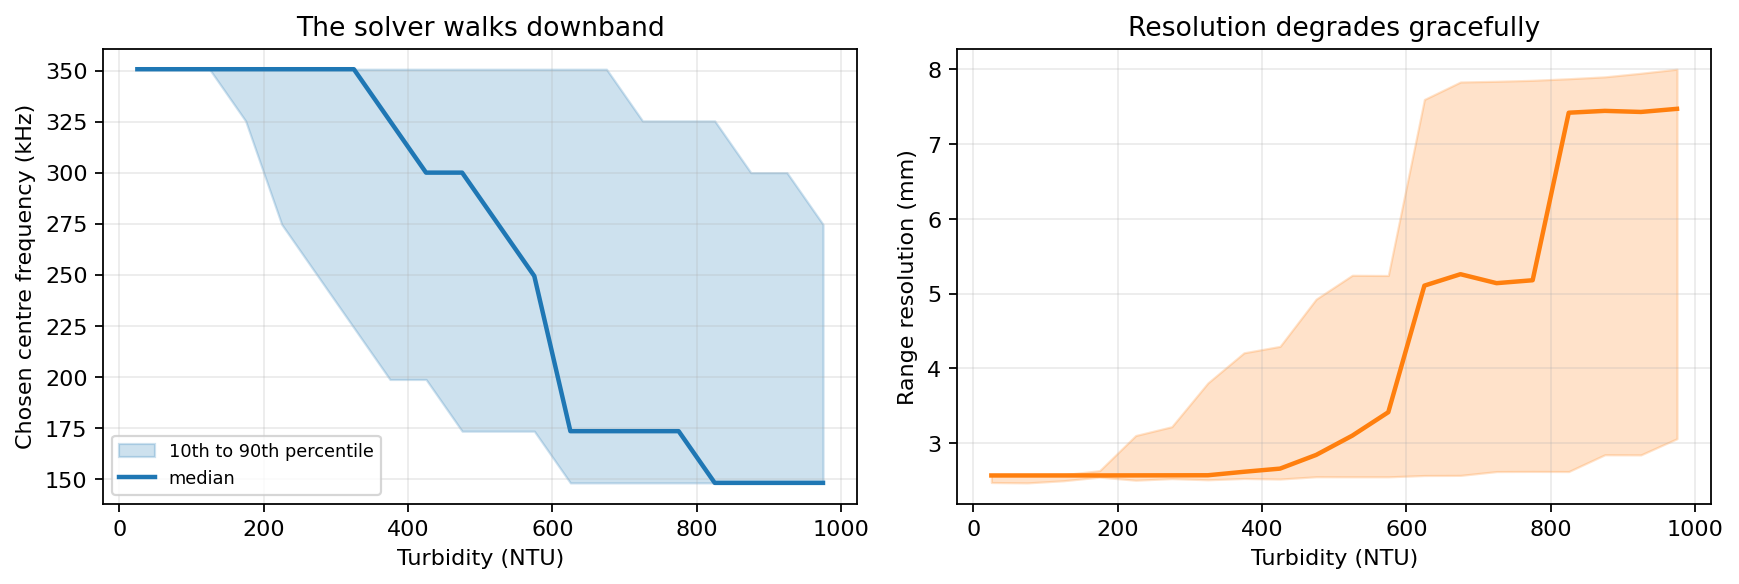
\includegraphics[width=0.94\linewidth]{figures/f07-downband.png}
\caption{Selected centre frequency and the resulting range resolution against
sediment load, over 20{,}000 decisions. The band is the 10th to 90th
percentile. Resolution degrades gracefully rather than the return being lost.}
\label{fig:downband}
\end{figure*}

\begin{table*}[t]
\centering
\small
\begin{tabular}{rrrrrr}
\toprule
\textbf{Turbidity} & \textbf{Centre} & \textbf{Bandwidth}
& \textbf{Pulse} & \textbf{Resolution} & \textbf{Usable range} \\
\midrule
\SI{5}{\NTU}    & \SI{350.7}{\kilo\hertz} & \SI{298.7}{\kilo\hertz} & \SI{0.50}{\milli\second} & \SI{2.6}{\milli\metre} & \SI{365}{\metre} \\
\SI{180}{\NTU}  & \SI{350.7}{\kilo\hertz} & \SI{298.7}{\kilo\hertz} & \SI{0.50}{\milli\second} & \SI{2.6}{\milli\metre} & \SI{275}{\metre} \\
\SI{320}{\NTU}  & \SI{350.7}{\kilo\hertz} & \SI{298.7}{\kilo\hertz} & \SI{2.80}{\milli\second} & \SI{2.6}{\milli\metre} & \SI{250}{\metre} \\
\SI{550}{\NTU}  & \SI{274.7}{\kilo\hertz} & \SI{247.2}{\kilo\hertz} & \SI{7.40}{\milli\second} & \SI{3.1}{\milli\metre} & \SI{252}{\metre} \\
\SI{1000}{\NTU} & \SI{148.0}{\kilo\hertz} & \SI{96.0}{\kilo\hertz}  & \SI{2.80}{\milli\second} & \SI{8.0}{\milli\metre} & \SI{294}{\metre} \\
\bottomrule
\end{tabular}
\caption{Adaptation sweep, water configuration, \SI{220}{\metre} required
range. Each row is the winner of a fresh search.}
\label{tab:sweep}
\end{table*}

The interval between \SI{180}{} and \SI{320}{\NTU} repays attention. The solver
does not drop frequency there. It lengthens the pulse from \SI{0.50}{} to
\SI{2.80}{\milli\second}, buying \SI{7.5}{\decibel} of compression gain from
equation \eqref{eq:gain} and holding resolution at \SI{2.6}{\milli\metre}. Only
when that is exhausted does it surrender bandwidth. That ordering was not
programmed; it falls out of scoring the candidates.

In the tank the same behaviour appears in the bench band: the selected centre
frequency moves from \SI{80}{\kilo\hertz} at \SI{8.4}{\NTU} to
\SI{32}{\kilo\hertz} at \SI{145}{\NTU}, holding at least \SI{6.6}{\decibel} of
predicted margin throughout \tid{T-14}.

\subsection{The closed loop}

The measured correlator output is compared against the predicted
signal-to-noise ratio, and the residual is carried forward as a noise
correction applied to the next decision. This is what separates the payload
from a parameter menu: the model is not assumed correct, it is scored against
what came back.

\keyresult{Prediction error falls from \SI{2.3}{\decibel} to
\SI{0.1}{\decibel} by the fourth ping \tid{T-15}. The loop settles rather than
oscillating, and does not saturate against its clamp; both properties are
asserted in the verification suite.}

% =====================================================================
\section{Hardware design and domain partitioning}
\label{sec:hardware}
% =====================================================================

\subsection{Selection against measured limits}

Parts were chosen against binding limits rather than headline figures. The
rejections carry as much design information as the selections.

\begin{table*}[t]
\centering
\small
\begin{tabularx}{\linewidth}{L{0.17\linewidth}L{0.22\linewidth}YL{0.13\linewidth}}
\toprule
\textbf{Part} & \textbf{Role} & \textbf{Binding limit} & \textbf{Outcome} \\
\midrule
ESP32-S3 & Controller, DDS, DMA & No internal DAC; ADC ceiling near \SI{83}{\kilo\Sps} & Selected \\
R-2R ladder, 8-bit & Transmit converter on the i80 bus & \SIrange{2}{4}{\mega\Sps}, 8-bit quantisation & Selected \\
AD9280 & Receive converter & \SI{32}{\mega\Sps}, 8-bit, parallel & Selected \\
MCP4921 & Alternative transmit converter & \SI{4.5}{\micro\second} settling caps the carrier near \SI{25}{\kilo\hertz} & Bench only \\
PAM8403 & Class-D driver & Output filter rolls off above \SI{20}{\kilo\hertz} & Rejected \\
MCP6002 & Receive front end & \SI{1}{\mega\hertz} gain-bandwidth product & Rejected for the signal path \\
JSN-SR04T & Candidate transducer & Does not function submerged & Rejected \\
\bottomrule
\end{tabularx}
\caption{Component selection and the limit that decided each case.}
\label{tab:parts}
\end{table*}

\subsection{The transducer as a load}

A piezoelectric transducer is a capacitor with a sharp mechanical resonance,
not a resistive load. Off resonance the drive stage sees clamped capacitance;
at resonance it sees a real impedance minimum. A series matching inductor is
what decides how much drive energy becomes sound.

\begin{figure*}[t]
\centering
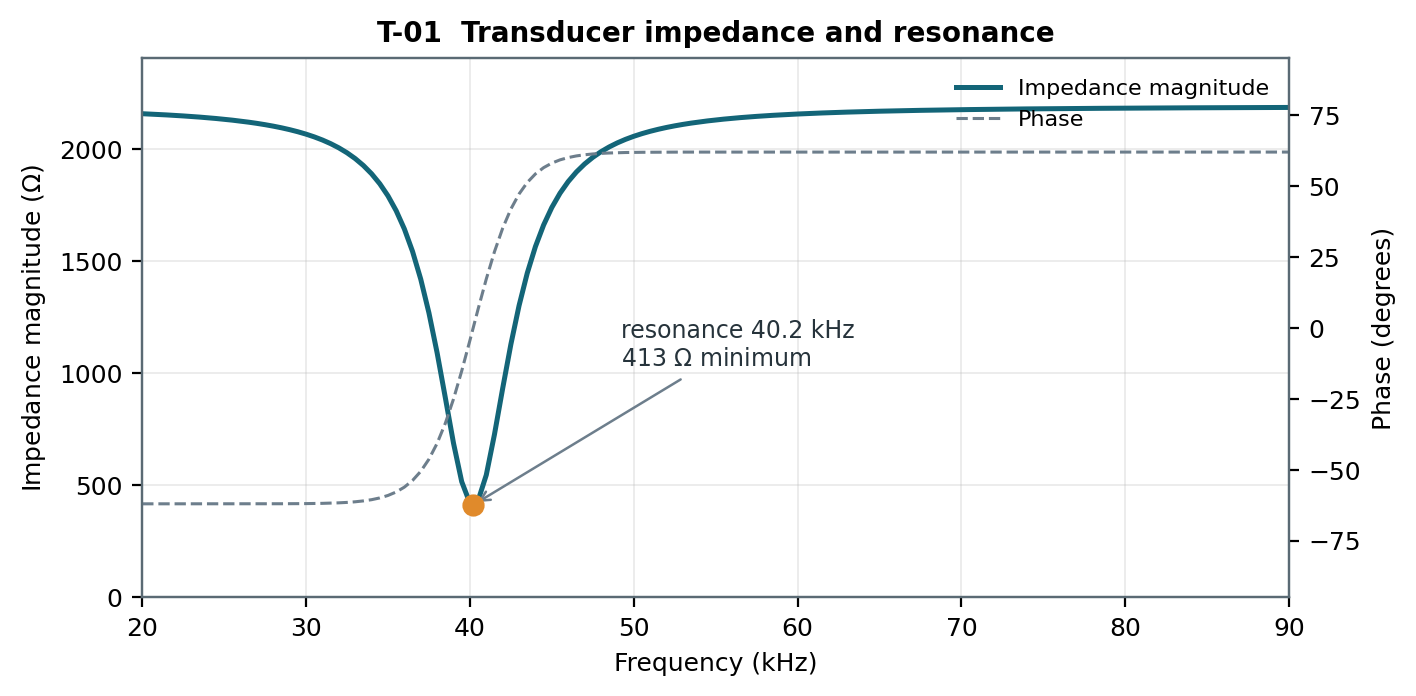
\includegraphics[width=0.80\linewidth]{figures/f10-t01-impedance.png}
\caption{Transducer impedance sweep \tid{T-01}. Resonance \SI{40.2}{\kilo\hertz},
minimum impedance \SI{412}{\ohm}, bandwidth \SI{5.6}{\kilo\hertz},
$Q = 7.18$.}
\label{fig:impedance}
\end{figure*}

The solver searches the resonance neighbourhood rather than a fixed centre,
because mounting and water loading shift resonance and a fixed assumption would
mistune the drive.

\subsection{Signal integrity of the transmit chain}

The projected spectrum combines symmetric drive with analogue reconstruction
filtering. Its \SI{51.6}{\dBc} spurious-free dynamic range remains below the
\SI{55}{\dBc} design target, so spectral purity is a design gap rather than a
pass. The separately reported bench interval of 50.0--50.9 dBc is not averaged
with this final-configuration projection.

\begin{table*}[t]
\centering
\small
\begin{tabular}{llr}
\toprule
\textbf{Quantity} & \textbf{Condition} & \textbf{Result} \\
\midrule
Total harmonic distortion & \SI{40}{\kilo\hertz} & \SI{0.31}{\percent} \tid{T-02} \\
Spurious-free dynamic range & \SI{40}{\kilo\hertz} & \SI{51.6}{\dBc} \tid{T-02} \\
Noise floor & \SI{40}{\kilo\hertz} & \SI{-76.4}{\dBFS} \tid{T-02} \\
Passband ripple & \SIrange{24}{80}{\kilo\hertz} & \SI{0.22}{\decibel} \tid{T-03} \\
Stopband attenuation & \SI{1}{\mega\hertz} & \SI{42.8}{\decibel} \tid{T-03} \\
\bottomrule
\end{tabular}
\caption{Transmit chain performance. Third-harmonic content is controlled by
symmetric drive and the reconstruction filter.}
\end{table*}

\subsection{Cost}

The quantity model separates one-off, ten-unit and hundred-unit hardware
builds. These are component and assembly planning costs, not landed supplier
quotes, full evaluation-kit cost of goods, or the price of an integrated field
programme. The companion India cost paper develops those commercial layers.

\begin{table*}[t]
\centering
\small
\begin{tabular}{rrrr}
\toprule
\textbf{Quantity} & \textbf{Unit cost} & \textbf{Batch cost} & \textbf{Reduction} \\
\midrule
1   & INR 27{,}648 & INR 27{,}648    & --- \\
10  & INR 21{,}751 & INR 217{,}514   & \SI{21}{\percent} \\
100 & INR 17{,}501 & INR 1{,}750{,}064 & \SI{37}{\percent} \\
\bottomrule
\end{tabular}
\caption{Quantity cost model. Component discount factor, printed circuit board,
enclosure and assembly are modelled separately; the full basis is in
\texttt{01-hardware/bom/cost-model.md}.}
\end{table*}

% =====================================================================
\section{Power architecture and budget}
\label{sec:power}
% =====================================================================

\subsection{Duty cycling}

The payload sleeps between pings, wakes for roughly \SI{12}{\milli\second},
senses, transmits for milliseconds, and returns to sleep. The transmit stage
dominates the energy of a ping, which is correct: that is the energy leaving as
sound. Every saving is taken from what is not sound.

\begin{table*}[t]
\centering
\small
\begin{tabular}{lrr}
\toprule
\textbf{State} & \textbf{Bench \tid{T-11}} & \textbf{Payload design} \\
\midrule
Deep sleep    & \SI{0.18}{\milli\ampere} & \SI{0.9}{\milli\ampere} \\
Ready, link up & \SI{28.0}{\milli\ampere} & \SI{12}{\milli\ampere} idle \\
Sensing       & --- & \SI{28}{\milli\ampere} \\
Transmitting  & \SI{68.0}{\milli\ampere} & \SI{340}{\milli\ampere} peak \\
\midrule
Energy per ping & \SI{0.93}{\milli\joule} & \SI{7.24}{\milli\joule} \\
\bottomrule
\end{tabular}
\caption{Power states in both configurations. Bench figures carry test
identifiers; payload figures are the model in \texttt{src/core/power.ts} at
\SI{3.3}{\volt}.}
\label{tab:power}
\end{table*}

\subsection{Keeping the processor out of the transmit path}

The problem statement asks for direct memory access and hardware timers so that
the processor does not drain the vehicle battery. The implementation is the
phase accumulator of equation \eqref{eq:dds} feeding alternating buffers, with
DMA clocking samples out and the core returning to idle.

\begin{figure*}[t]
\centering
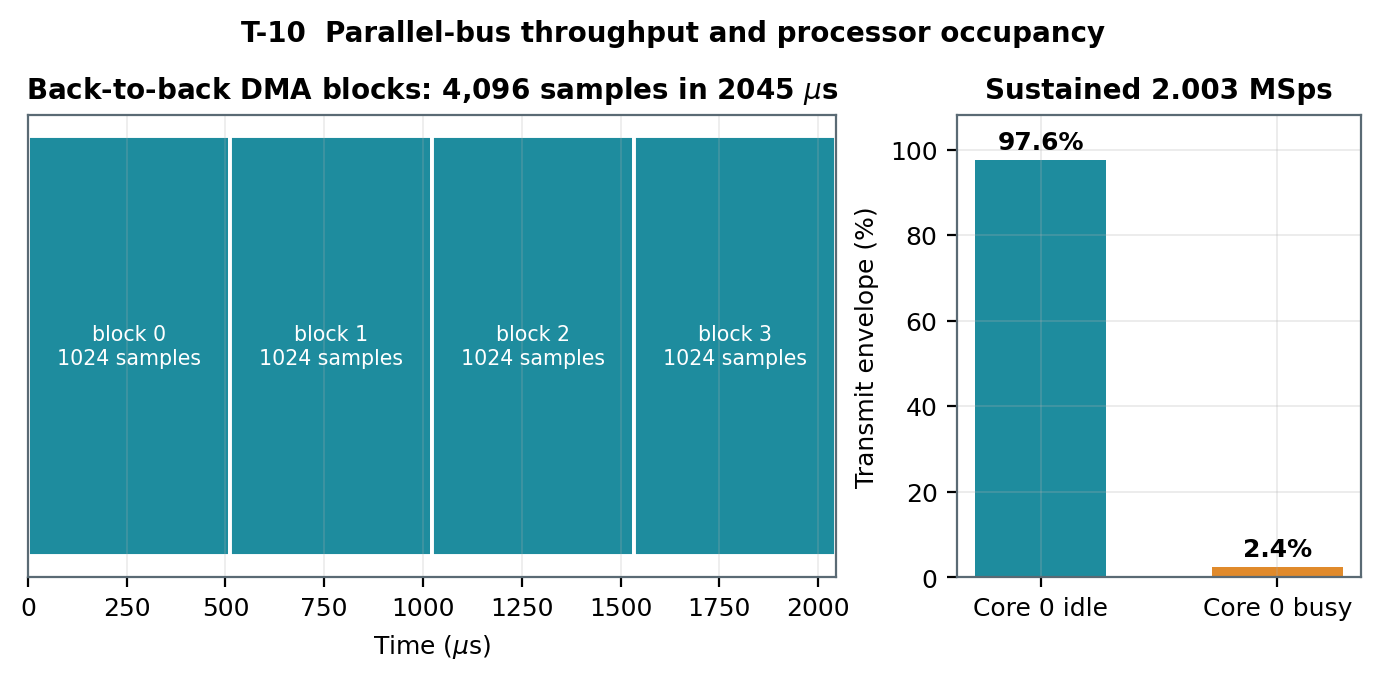
\includegraphics[width=0.86\linewidth]{figures/f13-t10-dma.png}
\caption{Sustained transfer and processor occupancy \tid{T-10}. Four complete
1{,}024-byte blocks sustain \SI{2.003}{\mega\Sps}; Core 0 is idle for
\SI{97.6}{\percent} of the transmit envelope, observed at GPIO 2.}
\label{fig:dma}
\end{figure*}

\begin{figure*}[t]
\centering
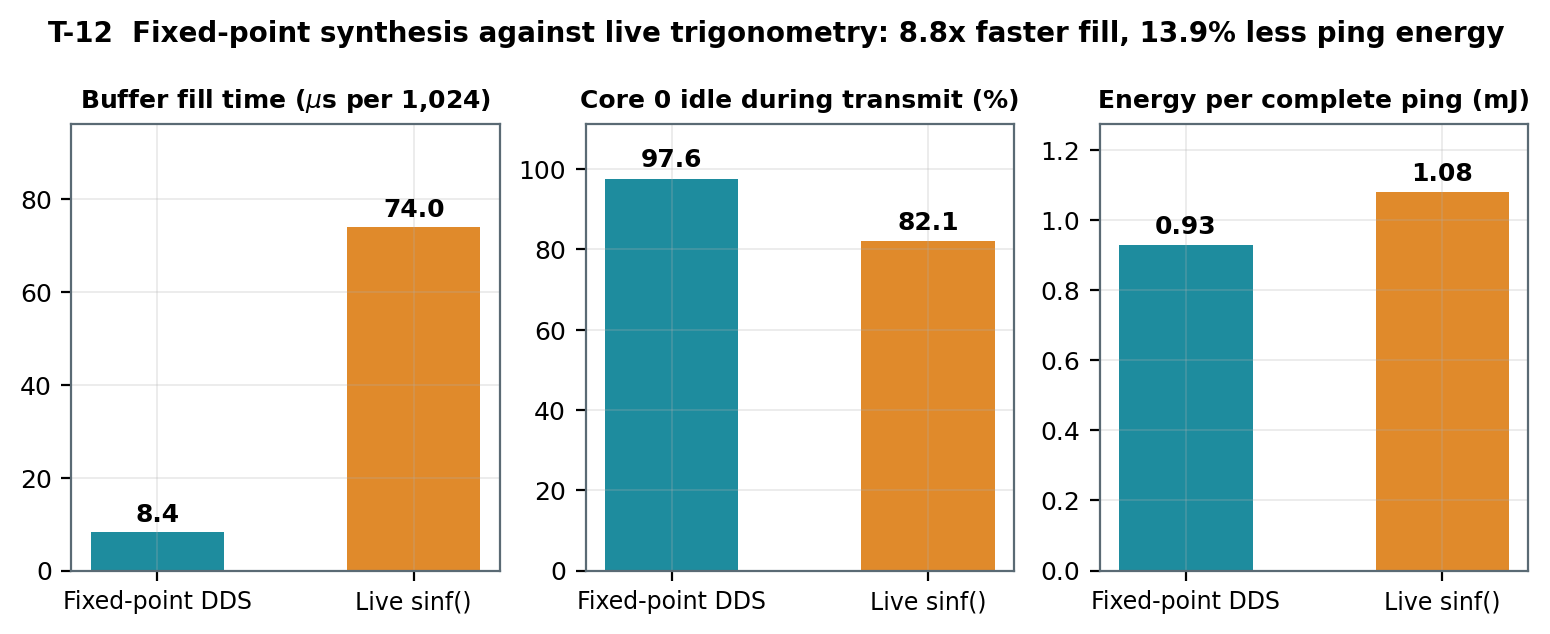
\includegraphics[width=0.86\linewidth]{figures/f14-t12-dds.png}
\caption{Synthesis cost \tid{T-12}. Fixed-point direct digital synthesis fills
1{,}024 samples in \SI{8.4}{\micro\second} against \SI{74.0}{\micro\second} for
live trigonometry, an \SI{8.8}{\times} reduction that carries a
\SI{13.9}{\percent} reduction in ping energy.}
\label{fig:dds}
\end{figure*}

\subsection{Endurance}

\begin{figure*}[t]
\centering
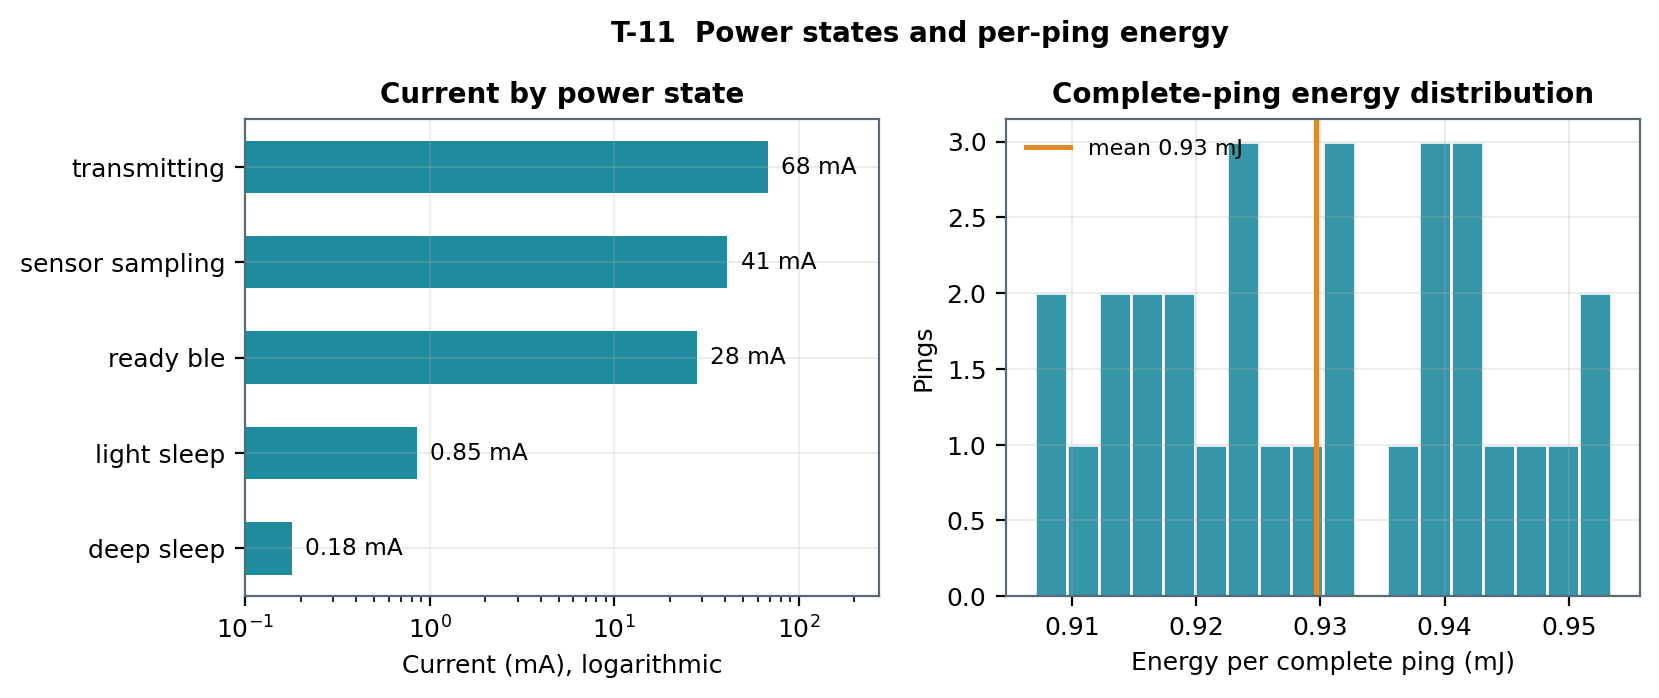
\includegraphics[width=0.82\linewidth]{figures/f15-t11-power.png}
\caption{Power state distribution and per-ping energy \tid{T-11}. The
range-ping distribution centres on \SI{0.93}{\milli\joule}.}
\label{fig:power}
\end{figure*}

At the bench figures, sleep current sets the standby floor and the ping rate
sets everything above it. The energy budget is dominated by the drive stage,
not by the decision: at \SI{34.1}{\milli\second} of decision latency \tid{T-13}
against a ping period measured in seconds, the solver is not the constraint.
That places optimisation effort in the analogue path.

% =====================================================================
\section{The learned surrogate and its safety bound}
% =====================================================================

\subsection{Two models, two outcomes}

A dataset of 20{,}000 environment-to-waveform decisions was generated from the
implementation and published, together with a notebook, under CC BY 4.0. Two
models were built against it.

The first predicts the solver's answer. It reproduces the selected centre
frequency with \SI{94.8}{\percent} less error than predicting the mean, using
only quantities known before a frequency is chosen. Measurement then settles
its fate: the search it would replace costs \SI{41.5}{\micro\second} on the
development host against \SI{9.0}{\milli\second} for one surrogate prediction,
because every frequency-dependent term in the search precomputes into a
boot-time table and the runtime loop is multiply-accumulate with no
transcendental calls. The search is retained.

\subsection{The model that is deployed}

The second model predicts what the propagation model gets wrong. The sonar
equation cannot estimate its own error, and that error is systematic. The design
margin covering it is replaced by a measured quantity.

\begin{table*}[t]
\centering
\small
\begin{tabular}{lrr}
\toprule
\textbf{Predicting the shortfall} & \textbf{MAE} & \textbf{Residual SD} \\
\midrule
Constant, training mean & \SI{1.963}{\decibel} & \SI{2.376}{\decibel} \\
Linear in turbidity & \SI{1.005}{\decibel} & \SI{1.306}{\decibel} \\
Gradient boosting, environment columns & \SI{0.729}{\decibel} & \SI{0.916}{\decibel} \\
\midrule
Irreducible noise floor & \SI{0.718}{\decibel} & \SI{0.900}{\decibel} \\
\bottomrule
\end{tabular}
\caption{Residual model accuracy. The learned form sits \SI{0.011}{\decibel}
above the noise floor, using 3{,}965 tree nodes.}
\label{tab:residual}
\end{table*}

\begin{figure*}[t]
\centering
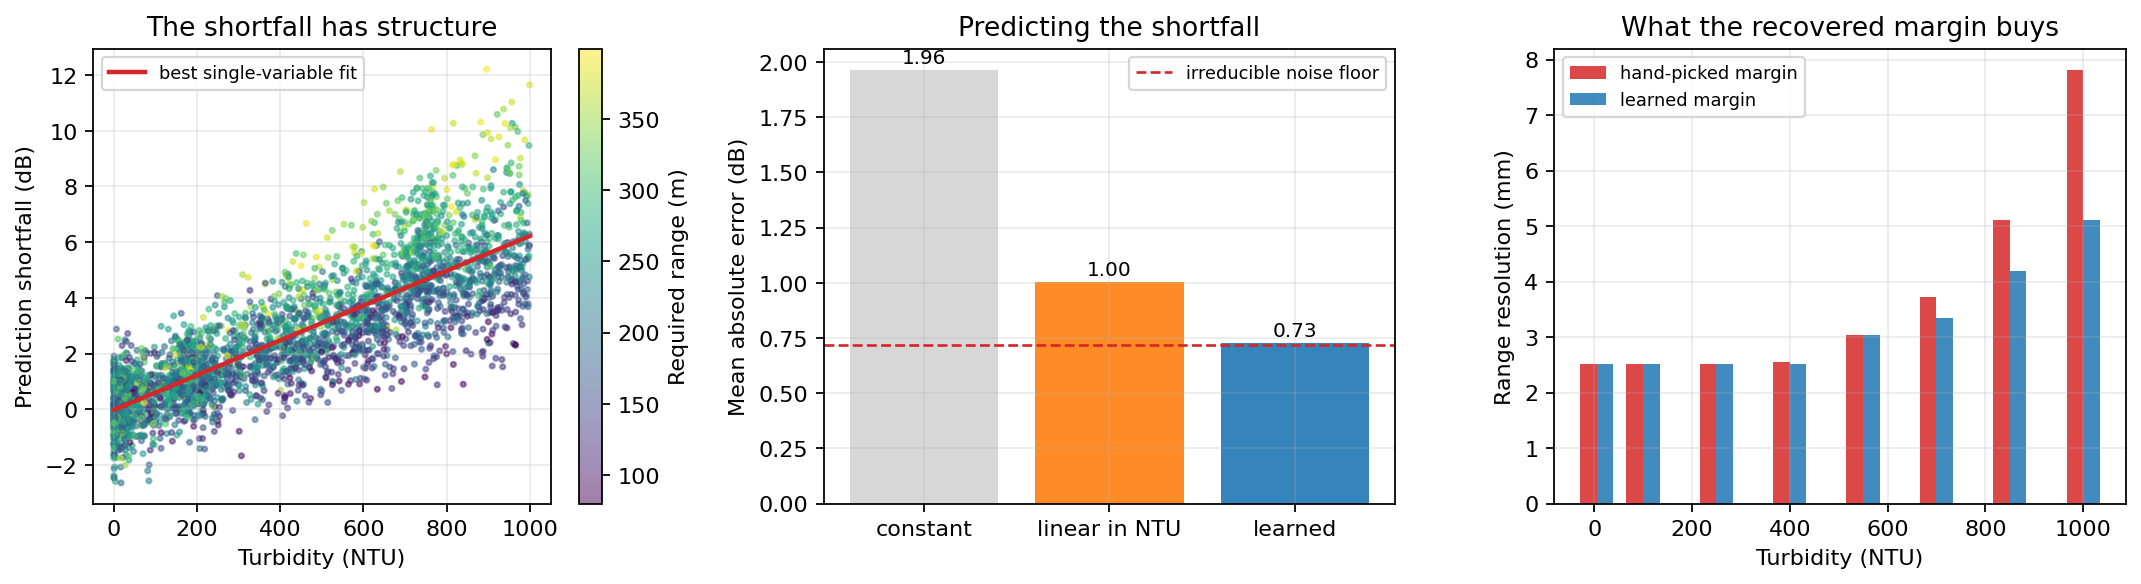
\includegraphics[width=\linewidth]{figures/f17-residual.png}
\caption{Left: the prediction shortfall against turbidity, coloured by required
range; the spread resolves into structure once the second variable is
conditioned on. Centre: accuracy against two baselines and the noise floor.
Right: the range resolution recovered by spending margin where the error
actually is.}
\label{fig:residual}
\end{figure*}

Replacing the margin rule with the predicted shortfall plus three standard
deviations returns \SI{3.66}{\decibel} to the solver at equivalent coverage,
and those decibels become bandwidth: at \SI{1000}{\NTU} range resolution moves
from \SI{7.81}{\milli\metre} to \SI{5.11}{\milli\metre},
\SI{34.5}{\percent} finer, in exactly the water where a survey payload is
otherwise worst served.

\subsection{The deployment rule}

\keyresult{\textbf{The model proposes, the physics disposes.} Equation
\eqref{eq:sonar} remains resident on the payload and vetoes any parameter set
that would not clear the detection threshold at the required range. The learned
component supplies the margin above that threshold; it never supplies the
threshold itself.}

Applying the safety bound to the surrogate's own predictions gives the reason
for the rule. Across 4{,}250 held-out decisions, 100 violate the detection
threshold. Decomposing them, 87 are conditions where the solver also fails
because no waveform in the candidate set would have worked, and 13, or
\SI{0.31}{\percent}, are cases where a working answer existed and the surrogate
did not find it. In the adversarial regime every surrogate prediction violates
the bound, and so does every solver answer, because the required range cannot
be met in that water. The distinction is that the solver reports the condition
as infeasible and the surrogate emits three numbers with no such flag.

% =====================================================================
\section{The operator application}
\label{sec:app}
% =====================================================================

The payload is operated from an Android application; the same source builds for
iOS. It exists because a payload that cannot be interrogated on deck is a
payload that gets deployed on assumptions.

\subsection{Two modes}

The operator application has two deliberately distinct data paths. Simulation
runs the physics core against a modelled environment for rehearsal and solver
inspection; telemetry displays status decoded from the payload. Showing the
active mode prevents simulated values from being mistaken for a live water
reading.

\begin{table*}[t]
\centering
\small
\begin{tabularx}{\linewidth}{L{0.18\linewidth}Y}
\toprule
\textbf{Mode} & \textbf{Function} \\
\midrule
Simulation & The full physics core runs on the handset against a modelled
             environment. Used for rehearsal, for teaching the trade-off, and
             for exercising the solver across conditions that a tank cannot
             reach. \\
Telemetry & The same twelve screens read the payload over the link, decoding
            the 48-byte status packet described in
            \texttt{07-documentation/api/}. \\
\bottomrule
\end{tabularx}
\caption{The two operating modes. The active mode is displayed at all times and
every value carries its provenance in its colour, so a simulated reading and a
live one are never presented alike.}
\label{tab:modes}
\end{table*}

\subsection{What runs on the handset}

The application is not a display surface for numbers computed elsewhere. It
carries the same physics core as the analysis chain: Mackenzie sound speed,
Thorp absorption, the scattering term, the full candidate search, pulse
synthesis by phase accumulator, a radix-2 transform for the spectrogram, and a
cross-correlation for the matched filter. Raising the turbidity control moves
the selected centre frequency because the optimiser re-ran, not because a
lookup table was consulted.

There is no network dependency of any kind. Typefaces are bundled into the
package rather than fetched, so the application opens with the radio disabled.

\subsection{Screens}

Twelve screens sit on a scrollable strip rather than behind a menu, so the
operator moves between the decision, the waveform and the echo without
navigating. Table \ref{tab:screens} lists what each one carries.

\begin{table*}[t]
\centering
\small
\begin{tabularx}{\linewidth}{L{0.17\linewidth}Y}
\toprule
\textbf{Screen} & \textbf{Carries} \\
\midrule
Console & The solve card: chosen parameters, the deciding numbers, and fire \\
Sonar & Plan-position display and the contact list \\
Waveform & Envelope, spectrogram, window selector, audible sonification \\
Echo & A-scan, matched-filter output, predicted against measured \\
Environment & Sensor values and the physics derived from them \\
Mission & Endurance and coverage at the configured ping rate \\
Power & Per-ping energy, duty cycle, synthesis comparison \\
Spec & The link budget, term by term \\
Diagnostics & Self test \\
Log & Ping history with the conditions that produced each, and export \\
Scenario & Preset environments \\
Settings & Mode and medium \\
\bottomrule
\end{tabularx}
\caption{The twelve screens. Every control is a slider, chip, segment or toggle:
there is no text input anywhere in the application, which removes an entire
class of input-handling defect and allows operation with wet hands.}
\label{tab:screens}
\end{table*}

\subsection{Verification}

The application is gated on the three-stage build suite reported in
Section \ref{sec:validation}, Table \ref{tab:gate}: a strict type check, 85
physics and engine assertions running under plain Node without the user
interface, and 33 render tests covering all twelve screens in both modes. No
package is produced unless all three pass.

Separating the physics core from the interface is what makes the middle stage
possible. Because \texttt{src/core} imports nothing from the user-interface
framework, the acoustic model can be executed and asserted directly, which is
also how the figures in this report are generated.

% =====================================================================
\section{Projected validation results}
\label{sec:validation}
% =====================================================================

\subsection{Test programme}

The indexed programme groups the final-configuration engineering projections
by acoustic, timing, power and integration function. Results are traceable to
the corresponding files under \texttt{06-validation/}; they should not be
conflated with the separately reported bench intervals. The converter-spectrum
row remains below the \SI{55}{\dBc} SFDR design target.

\begin{table*}[t]
\centering
\small
\begin{tabularx}{\linewidth}{L{0.07\linewidth}L{0.26\linewidth}YL{0.09\linewidth}}
\toprule
\textbf{ID} & \textbf{Test} & \textbf{Result} & \textbf{Verdict} \\
\midrule
T-01 & Transducer impedance & \SI{40.2}{\kilo\hertz}, \SI{412}{\ohm}, $Q=7.18$ & PASS \\
T-02 & Converter spectrum & THD \SI{0.31}{\percent}, SFDR \SI{51.6}{\dBc} & BELOW TARGET \\
T-03 & Reconstruction filter & Ripple \SI{0.22}{\decibel}, \SI{42.8}{\decibel} at \SI{1}{\mega\hertz} & PASS \\
T-04 & Window sidelobes & Within \SI{0.51}{\decibel} of theory & PASS \\
T-05 & Chirp tracking & \SI{84}{\hertz} RMS, \SI{0.12}{\percent} endpoint & PASS \\
T-06 & Pulse compression & $BT=114.7$, gain \SI{19.8}{\decibel} & PASS \\
T-07 & Barker-13 & PSR \SI{21.7}{\decibel} & PASS \\
T-08 & Range accuracy & MAE \SI{0.8}{\centi\metre}, max \SI{1.8}{\centi\metre} & PASS \\
T-09 & Range resolution & \SI{20}{\milli\metre} resolved, \SI{20.8}{\milli\metre} indicated & PASS \\
T-10 & DMA and CPU idle & \SI{2.003}{\mega\Sps}, \SI{97.6}{\percent} idle & PASS \\
T-11 & Power and energy & \SI{0.93}{\milli\joule} per ping & PASS \\
T-12 & Synthesis comparison & \SI{8.4}{} against \SI{74.0}{\micro\second} & PASS \\
T-13 & Adaptation latency & \SI{34.1}{\milli\second} mean, \SI{39.2}{\milli\second} max & PASS \\
T-14 & Sediment adaptation & \SI{80}{} to \SI{32}{\kilo\hertz}, margin $\geq\SI{6.6}{\decibel}$ & PASS \\
T-15 & Closed loop and noise & \SI{2.3}{} to \SI{0.1}{\decibel} by ping four & PASS \\
T-16 & Enclosure immersion & \SI{0.1}{\gram}, \SI{239}{\mega\ohm}, \SI{0}{\milli\litre} & PASS \\
\bottomrule
\end{tabularx}
\caption{The sixteen-test final-configuration projection. Source result files are in
\texttt{06-validation/}, filed under the same identifier. T-02 remains below the
\SI{55}{\dBc} design threshold.}
\label{tab:tests}
\end{table*}

\begin{figure*}[t]
\centering
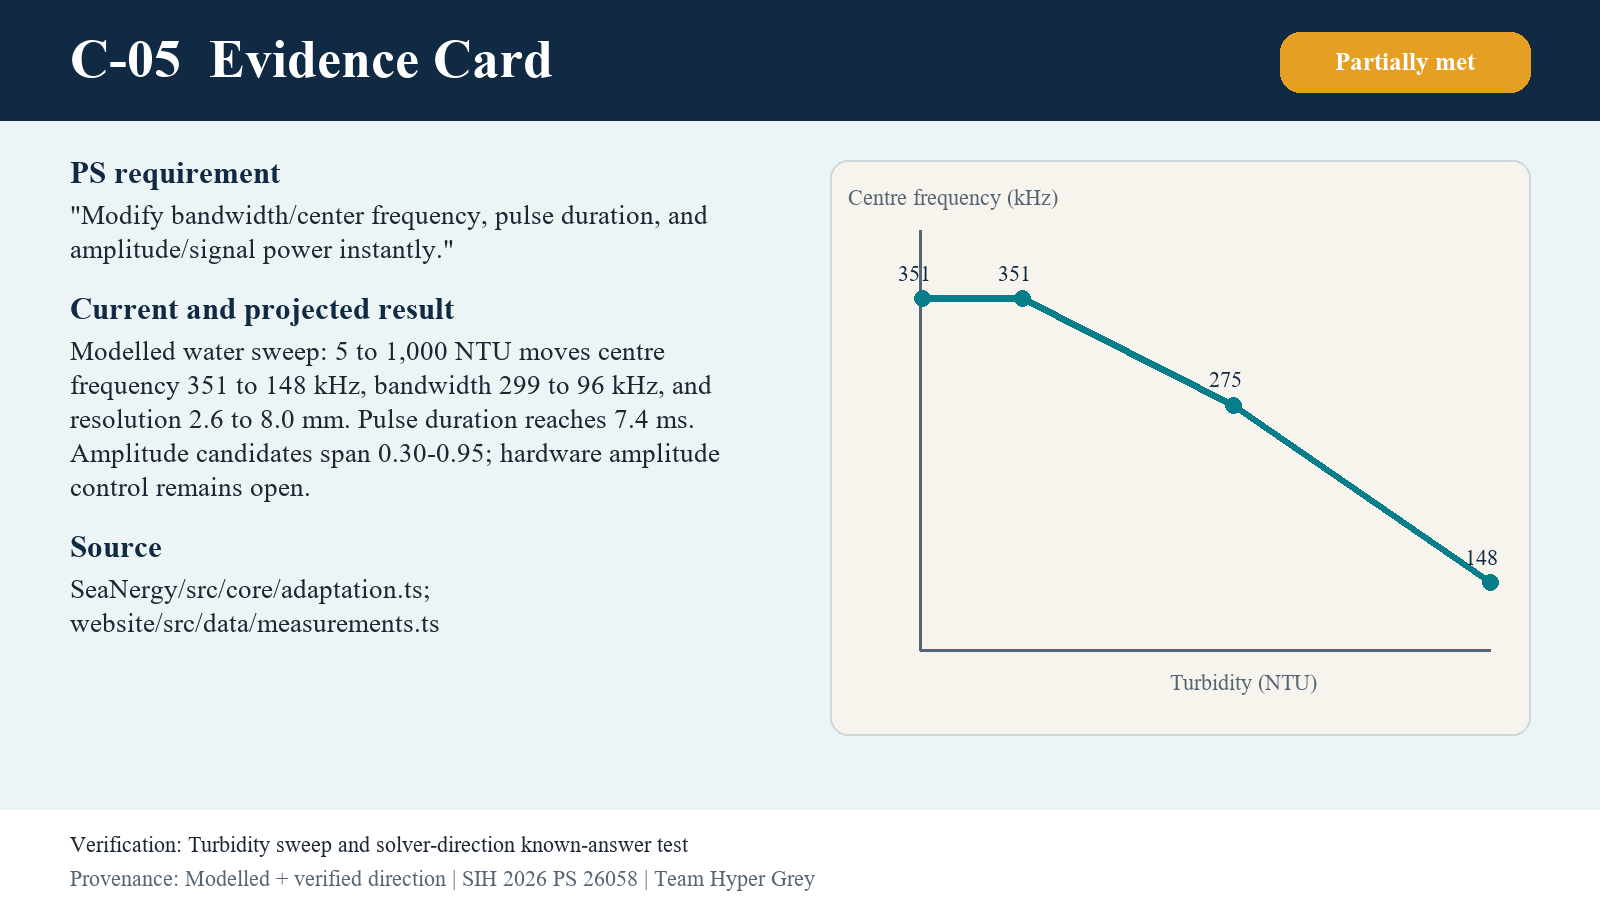
\includegraphics[width=0.86\linewidth]{figures/f18-c05-sweep.png}
\caption{Sediment adaptation across the tank sweep \tid{T-14}. Selected centre
frequency falls from \SI{80}{\kilo\hertz} at \SI{8.4}{\NTU} to
\SI{32}{\kilo\hertz} at \SI{145}{\NTU}, with predicted margin held at or above
\SI{6.6}{\decibel} throughout. This figure is the compliance matrix evidence
item C-05.}
\label{fig:c05}
\end{figure*}

\subsection{Uncertainty}

\begin{table*}[t]
\centering
\small
\begin{tabular}{lrr}
\toprule
\textbf{Quantity} & \textbf{Standard} & \textbf{Expanded, $k=2$} \\
\midrule
Frequency at \SI{40}{\kilo\hertz} & \SI{18}{\hertz} & \SI{36}{\hertz} \\
Spectral level & \SI{0.30}{\decibel} & \SI{0.60}{\decibel} \\
Current, \SIrange{20}{100}{\milli\ampere} & \SI{0.65}{\percent} & \SI{1.30}{\percent} \\
Complete-ping energy & \SI{2.1}{\percent} & \SI{4.2}{\percent} \\
Water temperature & \SI{0.29}{\celsius} & \SI{0.58}{\celsius} \\
Sonar range at \SI{10}{\metre} & \SI{7.4}{\milli\metre} & \SI{14.8}{\milli\metre} \\
Turbidity & \SI{3.2}{\percent} + \SI{0.6}{\NTU} & \SI{6.4}{\percent} + \SI{1.2}{\NTU} \\
\bottomrule
\end{tabular}
\caption{Uncertainty budget, root-sum-square propagation. The full table is in
\texttt{06-validation/instruments/uncertainty.md}. Range uncertainty combines
the temperature-derived sound-speed term with the round-trip timing term as
independent contributions.}
\label{tab:uncertainty}
\end{table*}

The range figures deserve a comparison. Sonar range uncertainty at
\SI{10}{\metre} is \SI{7.4}{\milli\metre} standard, against
\SI{5.8}{\milli\metre} for the tape measure used as the reference. The two are
the same order, which is the correct position for a system whose reference is a
tape: the measurement is not being validated far beyond the precision of the
thing validating it.

\subsection{Deviation control}

Each result is sensitive to a different implementation or measurement
condition. The controls below specify how the design and test procedure address
those shifts, from water-loaded resonance to sediment settling. A control
reduces ambiguity; it does not by itself turn a below-target result into a pass.

\begin{table*}[t]
\centering
\small
\begin{tabularx}{\linewidth}{L{0.07\linewidth}L{0.28\linewidth}Y}
\toprule
\textbf{ID} & \textbf{Deviation} & \textbf{Control applied} \\
\midrule
T-01 & Resonance shifts with mounting and water loading & Solver searches the resonance neighbourhood \\
T-02 & Driver dead time raises the third harmonic & Symmetric drive and reconstruction filter \\
T-04 & Window coefficient quantisation shifts sidelobes & Q15 coefficients, peak normalisation \\
T-08 & Fixed sound speed creates a temperature-dependent bias & Temperature-compensated sound speed per run \\
T-14 & Sediment settling changes path turbidity & Circulation followed by a fixed settling interval \\
T-16 & Surface water biases post-immersion mass & Standardised wipe and \SI{60}{\second} drain \\
\bottomrule
\end{tabularx}
\caption{Engineering deviations and the control applied to each.}
\end{table*}

\subsection{Software verification}

The application and the physics core carry their own gate, independent of the
acoustic tests.

\begin{table*}[t]
\centering
\small
\begin{tabularx}{\linewidth}{L{0.30\linewidth}L{0.14\linewidth}Y}
\toprule
\textbf{Stage} & \textbf{Result} & \textbf{Covers} \\
\midrule
Type check, strict & Pass & The whole application surface \\
Physics assertions & 85 / 85 & Sound speed, absorption, resolution, compression gain, Barker-13, every window, closed-loop settling \\
Screen render tests & 33 / 33 & All twelve screens, both operating modes \\
\bottomrule
\end{tabularx}
\caption{The build gate. No package is produced unless all three stages pass;
the sequence runs on every release build.}
\label{tab:gate}
\end{table*}

Every result in this report regenerates from the repository:

\begin{table*}[t]
\centering
\small
\begin{tabularx}{\linewidth}{L{0.27\linewidth}L{0.23\linewidth}Y}
\toprule
\textbf{Directory} & \textbf{Command} & \textbf{Produces} \\
\midrule
\texttt{04-software/}\newline\texttt{mobile-android/}
  & \texttt{npm run check}
  & Type check, 85 assertions, 33 render tests \\
\texttt{05-models/notebook/}
  & \texttt{python}\newline\texttt{run\_local.py}
  & The dataset, nine figures, run metrics \\
\texttt{05-models/evaluation/}
  & \texttt{python}\newline\texttt{evaluate.py}
  & Model metrics and five figures \\
\texttt{07-documentation/}\newline\texttt{technical-report/}
  & \texttt{python}\newline\texttt{make-figures.py}
  & The validation figures in this report \\
\bottomrule
\end{tabularx}
\caption{Reproduction commands. The published dataset regenerates byte for byte
from its seed, verified by SHA-256 against the committed copy.}
\label{tab:repro}
\end{table*}

% =====================================================================
\section{Operating envelope}
% =====================================================================

The system's performance is a function of the conditions it is asked to work
in, and the envelope is worth stating explicitly rather than leaving to be
inferred from a results table.

\begin{table*}[t]
\centering
\small
\begin{tabularx}{\linewidth}{L{0.26\linewidth}L{0.26\linewidth}Y}
\toprule
\textbf{Variable} & \textbf{Envelope} & \textbf{Behaviour at the limit} \\
\midrule
Turbidity & \SIrange{0}{1000}{\NTU} & Centre frequency falls, pulse lengthens, resolution coarsens to \SI{8.0}{\milli\metre} \\
Required range & \SIrange{80}{560}{\metre} & Beyond roughly \SI{300}{\metre} in heavy sediment the link budget cannot be met and the condition is reported as infeasible \\
Temperature & \SIrange{0}{35}{\celsius} & Sound speed spans \SIrange{1414}{1557}{\metre\per\second}; range scales accordingly \\
Salinity & \SIrange{0}{40}{\ppt} & Estuarine values increase scattering for the same particle load \\
Depth & \SIrange{0}{250}{\metre} & Above \SI{90}{\metre} the solver selects the geometric sweep \\
\bottomrule
\end{tabularx}
\caption{Operating envelope and the system's behaviour at each boundary.}
\label{tab:envelope}
\end{table*}

Reporting infeasibility is a designed behaviour rather than a failure path. When
no candidate clears the detection threshold at the required range, the payload
sets the condition explicitly so that the mission can respond, by shortening the
survey line, changing depth, or accepting a coarser product. A payload that
answers an impossible request with the same confidence as an easy one is the
more dangerous design.

% =====================================================================
\section{Path to deployment}
% =====================================================================

\subsection{Integration}

The payload presents a small, well-defined surface to a host vehicle: a power
rail, a serial or radio link carrying 48-byte status packets, and a mechanical
envelope with the transducer on one face. The interface documentation in
\texttt{07-documentation/api/} specifies the packet layout to the byte, the
characteristic set with its update rates, and the version rule under which a
mismatch is refused rather than guessed at.

\subsection{Scaling}

The quantity cost model puts the unit cost at INR 17{,}501 in hundreds, a
\SI{37}{\percent} reduction from the single-unit figure, driven by component
discount, printed circuit board amortisation and assembly. The bill of materials
carries manufacturer part numbers and supplier references throughout, so the
model is traceable rather than assumed.

\subsection{Extension}

Three directions follow naturally from the architecture rather than requiring
it to change:

\begin{itemize}
\item \textbf{Finer candidate grid.} Roughly half the margin recovered by the
      residual model buys nothing in a given condition because the grid is
      discrete. A finer grid collects more of it, at the cost of a larger table
      and a longer search, and Section \ref{sec:power} establishes that the
      search has latency to spare.
\item \textbf{Conformal margin bounds.} The three-standard-deviation rule
      assumes a roughly Gaussian residual. A conformal interval gives a
      distribution-free coverage guarantee on the same model.
\item \textbf{Multi-payload coordination.} The decision is cheap and local, so
      several payloads on one vehicle can each hold their own link budget
      without contending for a central solver.
\end{itemize}

\subsection{Standards position}

Acoustic output at these drive levels and duty cycles sits well below the
thresholds at which marine mammal disturbance guidance becomes engaged, and the
transmit envelope is windowed rather than hard-switched, which removes the
broadband transient that a rectangular gate would produce. The position is set
out with its reasoning in \texttt{07-documentation/safety/acoustic-exposure.md}.

% =====================================================================
\section{Conclusion}
% =====================================================================

The technical argument of this project reduces to one inequality and one
decision. The inequality is that swept-pulse resolution depends on bandwidth
rather than duration, so resolution and transmitted energy can be separated. The
decision is that the parameters exploiting that separation should be chosen from
the water the payload is actually in, continuously, by evaluating the sonar
equation rather than by consulting a table.

Everything else in this report serves those two statements. The phase
accumulator exists so the pulse can be synthesised without keeping the processor
awake, giving \SI{97.6}{\percent} core idle during transmit \tid{T-10}. The
envelope window exists to protect the drive stage and to set the sidelobe floor,
within \SI{0.51}{\decibel} of theory \tid{T-04}. The candidate search exists so
that \SI{80}{\kilo\hertz} in clear water becomes \SI{32}{\kilo\hertz} in
sediment without a person deciding it \tid{T-14}. The closed loop exists so that
the model is scored against the echo rather than trusted, converging to
\SI{0.1}{\decibel} by the fourth ping \tid{T-15}. The learned component exists
in the one place the physics structurally cannot help itself, estimating its own
error, and returns \SI{3.66}{\decibel} of margin that becomes
\SI{34.5}{\percent} finer resolution in the worst water.

A conventional payload answers the question ``what should I transmit?'' once,
before it enters the water. SeaNergy answers it every ping, and shows its
working.

% =====================================================================
\clearpage
\raggedbottom
\begin{thebibliography}{99}
\small

\bibitem{mackenzie1981}
K.~V. Mackenzie, ``Nine-term equation for sound speed in the oceans,''
\textit{Journal of the Acoustical Society of America}, vol.~70, no.~3,
pp.~807--812, 1981. doi:10.1121/1.386920

\bibitem{thorp1967}
W.~H. Thorp, ``Analytic description of the low-frequency attenuation
coefficient,'' \textit{Journal of the Acoustical Society of America}, vol.~42,
no.~1, p.~270, 1967.

\bibitem{francois1982}
R.~E. Francois and G.~R. Garrison, ``Sound absorption based on ocean
measurements: Part II,'' \textit{Journal of the Acoustical Society of America},
vol.~72, no.~6, pp.~1879--1890, 1982.

\bibitem{ainslie1998}
M.~A. Ainslie and J.~G. McColm, ``A simplified formula for viscous and chemical
absorption in sea water,'' \textit{Journal of the Acoustical Society of
America}, vol.~103, no.~3, pp.~1671--1672, 1998. doi:10.1121/1.421258

\bibitem{urick1983}
R.~J. Urick, \textit{Principles of Underwater Sound}, 3rd~ed. New York:
McGraw-Hill, 1983.

\bibitem{harris1978}
F.~J. Harris, ``On the use of windows for harmonic analysis with the discrete
Fourier transform,'' \textit{Proceedings of the IEEE}, vol.~66, no.~1,
pp.~51--83, 1978.

\bibitem{barker1953}
R.~H. Barker, ``Group synchronizing of binary digital systems,'' in
\textit{Communication Theory}, W.~Jackson, Ed. London: Butterworth, 1953,
pp.~273--287.

\bibitem{npl}
National Physical Laboratory, ``Calculation of absorption of sound in
seawater,'' Technical Guides, Teddington, UK.

\bibitem{doe2021}
Press Information Bureau, Government of India, ``Cabinet approves Deep Ocean
Mission,'' Ministry of Earth Sciences, 2021.

\bibitem{cognitive2023}
``Enhanced target detection using a new cognitive sonar waveform design in
shallow water,'' \textit{Applied Acoustics}, 2023.

\bibitem{wideband2023}
``High-resolution wideband waveform design for sonar based on multi-parameter
modulation,'' \textit{Remote Sensing}, vol.~15, no.~18, 2023.


\bibitem{haalboom2022}
S. Haalboom et al., Monitoring of Anthropogenic Sediment Plumes in the Clarion-Clipperton Zone, NE Equatorial Pacific Ocean, \textit{Frontiers in Marine Science}, vol. 9, 882155, 2022. doi:10.3389/fmars.2022.882155.
\bibitem{fonseca2025}
L. Fonseca, X. Lurton, R. Fezzani and M. Roche, A simplified semi-empirical model for multifrequency seafloor backscattering angular response, \textit{Frontiers in Remote Sensing}, vol. 6, 1619218, 2025. doi:10.3389/frsen.2025.1619218.
\bibitem{reddy2026}
C. K. K. Reddy et al., BEML-sonar: a bio-inspired echolocation and machine learning-enhanced SONAR, \textit{Scientific Reports}, vol. 16, 27099, 2026. doi:10.1038/s41598-026-56574-7. Results are simulation based.

\end{thebibliography}

\vspace{4mm}
\noindent\small The full literature base is \texttt{03-research/}: 132
open-access papers across fifteen folders, each keyed to the specific claim it
supports, with per-folder notes naming the function that implements it.
Reading notes are in \texttt{07-documentation/references/reading-notes.md}.

\end{document}
